This section displays the CNN variations of the CNN, their accuracy's and comments on their run time, which impeding the projects progress greatly. The types of CNN variations testing were done out of sequence and sorted, reordered into this section.

\section{All Subjects, Session 1 to 7 Classification}
\label{All Subjects, Session 1 to 7 Classification Section}

When testing session 1 to 7, all subjects, the test accuracy placed into a separate spreadsheet where an average accuracy was calculated using the best accuracy's for each subject (the best of the 7 sessions) such as was done to achieve the project objective of 76\% (\cite{PalaniPaper}). All the test accuracy's in this sections are given using the average of best accuracy's.

\subsection{Testing the Epochs}
\label{All Subjects, 1 to 7 TestEpoch}

By running each experiment 3 times, an average test accuracy can be formed. Using the same CNN variation used in \cite{PalaniPaper}, \cref{S1-7 50 Epochs Acc} shows 3 runs of this CNN variation at 50 epochs. These 3 runs gave an average of test accuracy of 78.18\% with the highest at 78.53\% and the lowest at 77.47\%. Changing the CNN to 30 epochs shown in \cref{S1-7 30 Epochs Acc} which the highest accuracy was 79.07\% and the lowest at 78.67\% which again out of 3 run gave an average of 78.94\%. Lowering the number of epochs slightly increased the accuracy but not by a margin considerably to justify lowering the variation to 30 epochs. To further evaluate this, \cref{S1-7 Varied Epochs Acc} indicates that lowering the epochs to 11 gave 74.27\% and 1 epoch at 41.72\%, this follows the logic that a higher number of epochs allows more cycles of the training data and therefore train the CNN more to produce higher, more efficient test accuracy. One benefit to lowering the max epoch was a faster run time, the 50 epoch runs completed in around 7 hours 50 minutes and 30 epoch runs, 4 hours 47 minutes. 

\begin{figure}[H]
\centering
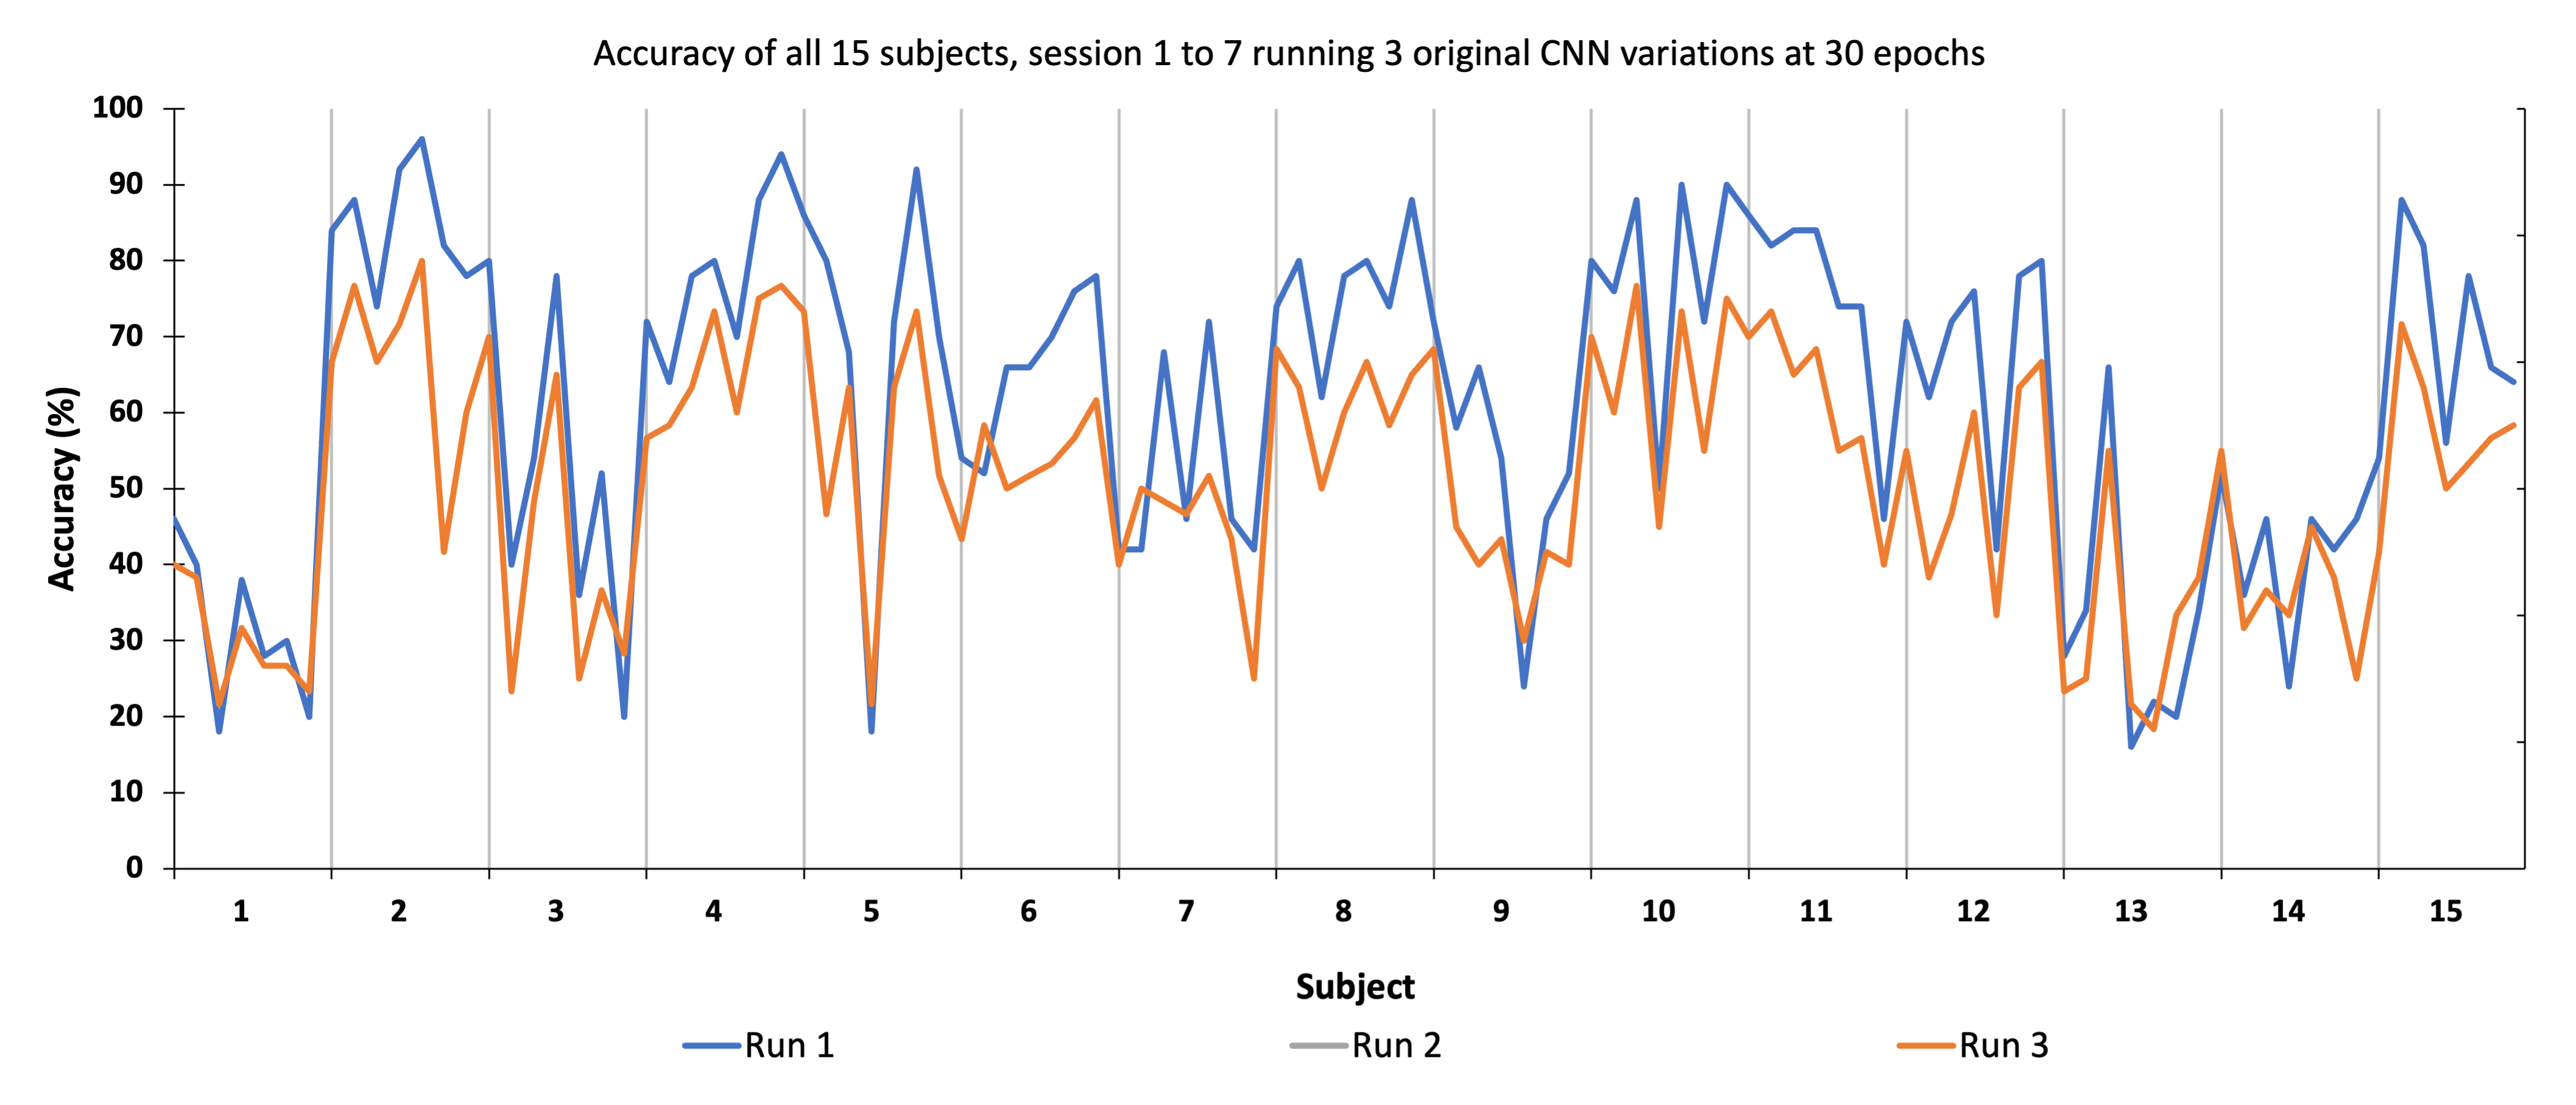
\includegraphics[scale=0.5]{Media/SBJ1-15_S1-7/SBJ1-15&S1-7_3_Runs_30_Epochs_Accuracy.png}
\caption{Test accuracy for all 105 sessions across all 15 subjects, comparing 3 runs of the CNN variation of changing the max epochs from 50 to 30.}
\label{S1-7 30 Epochs Acc}
\end{figure}

\begin{figure}[H]
\centering
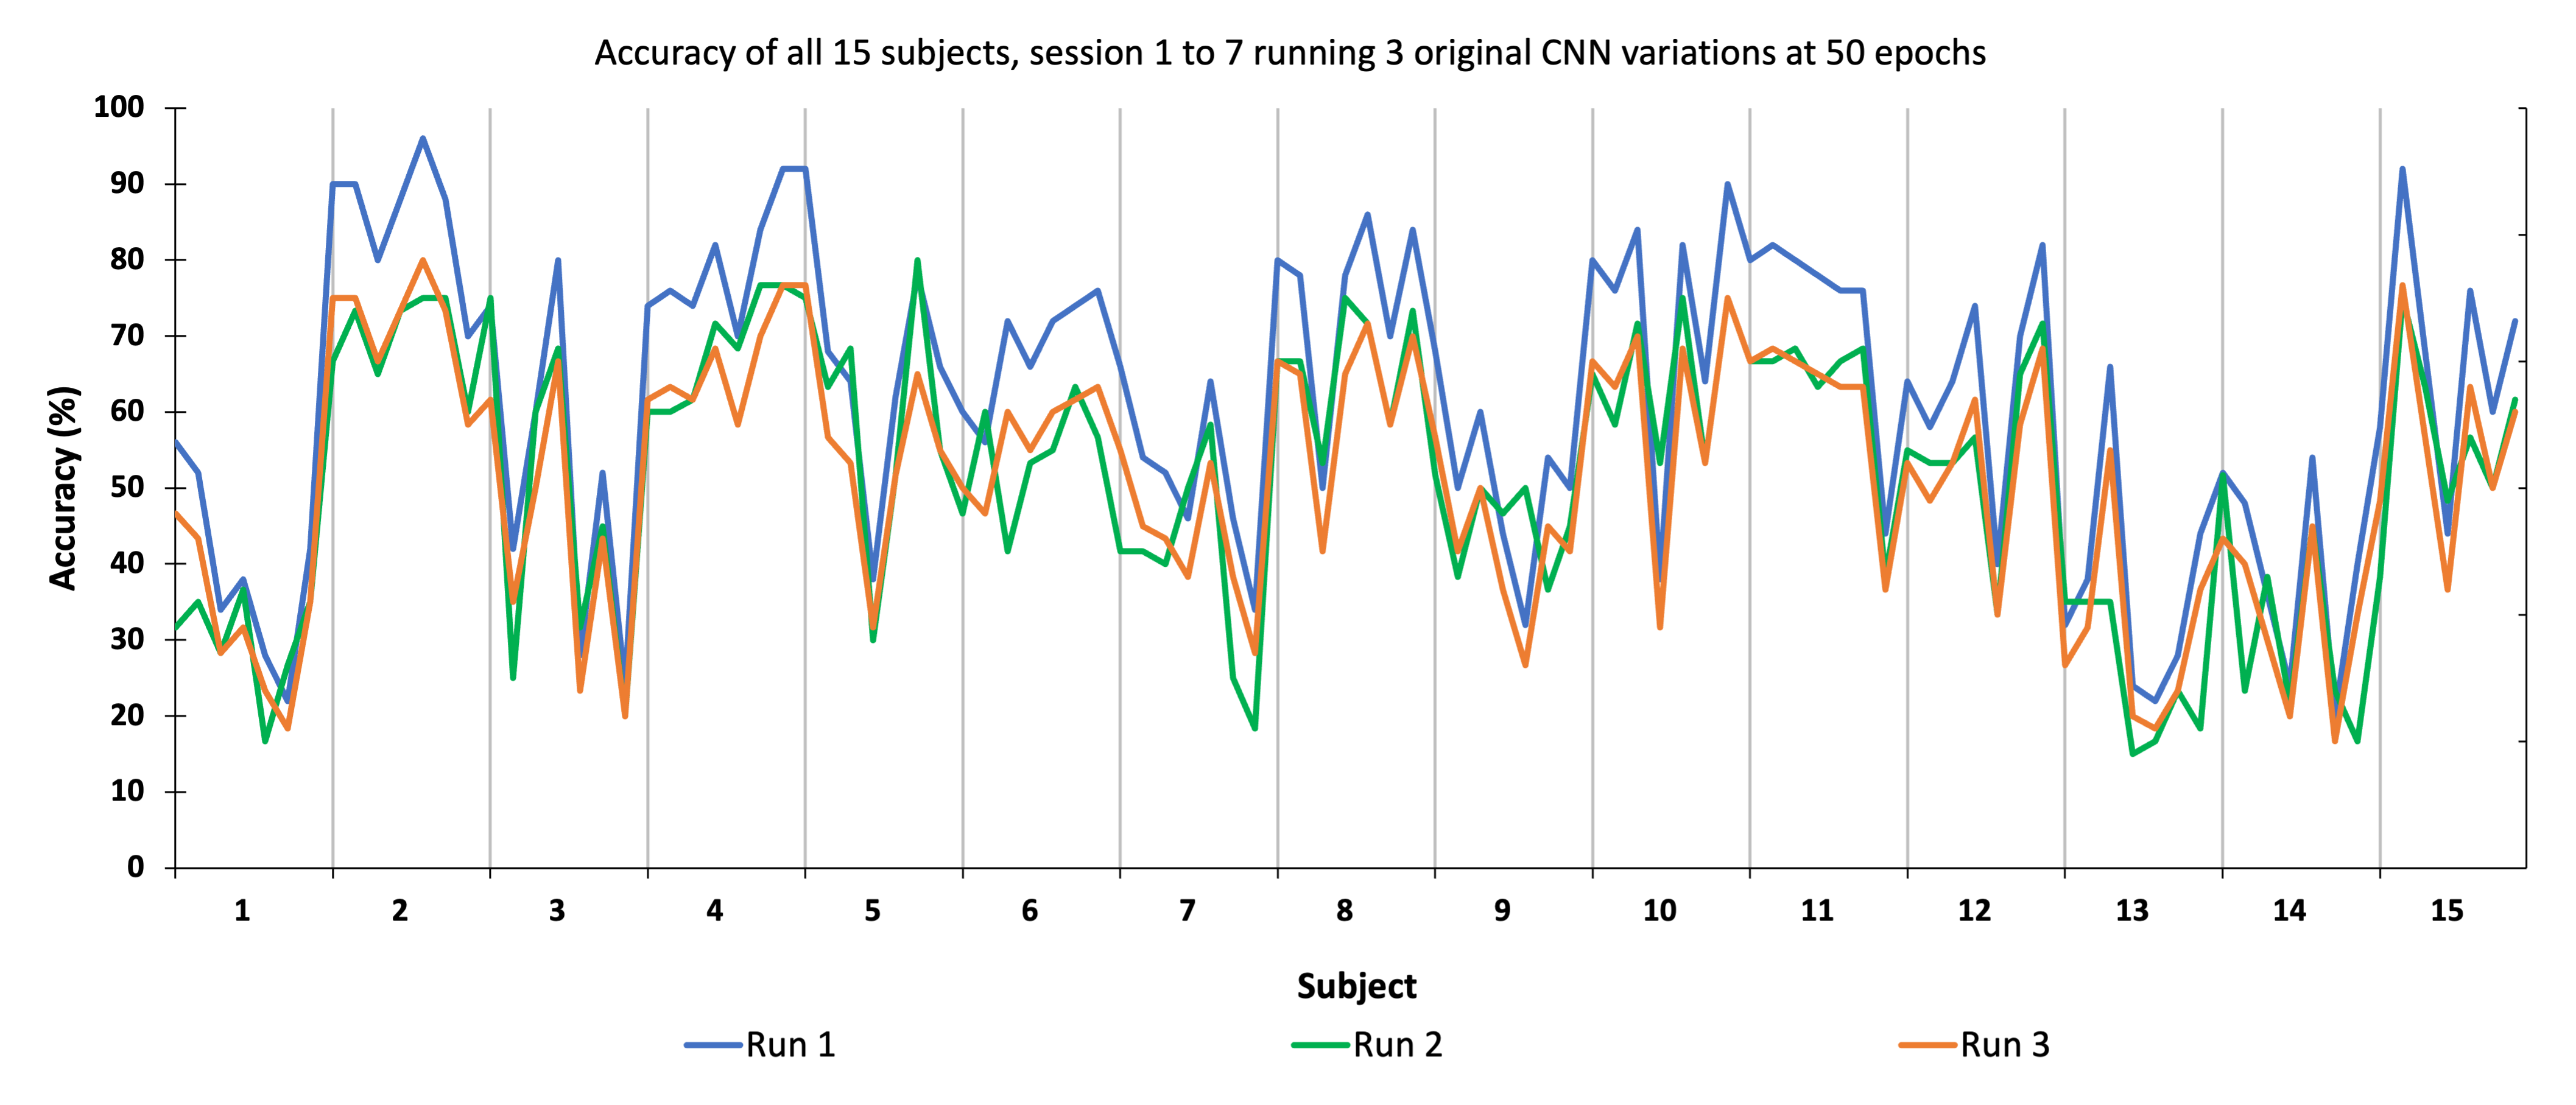
\includegraphics[scale=0.5]{Media/SBJ1-15_S1-7/SBJ1-15&S1-7_3_Runs_50_Epochs_Accuracy.png}
\caption{Test accuracy for all 105 sessions across all 15 subjects, comparing 3 runs of the original CNN variation used in (\cite{PalaniPaper}).}
\label{S1-7 50 Epochs Acc}
\end{figure}

\begin{figure}[H]
\centering
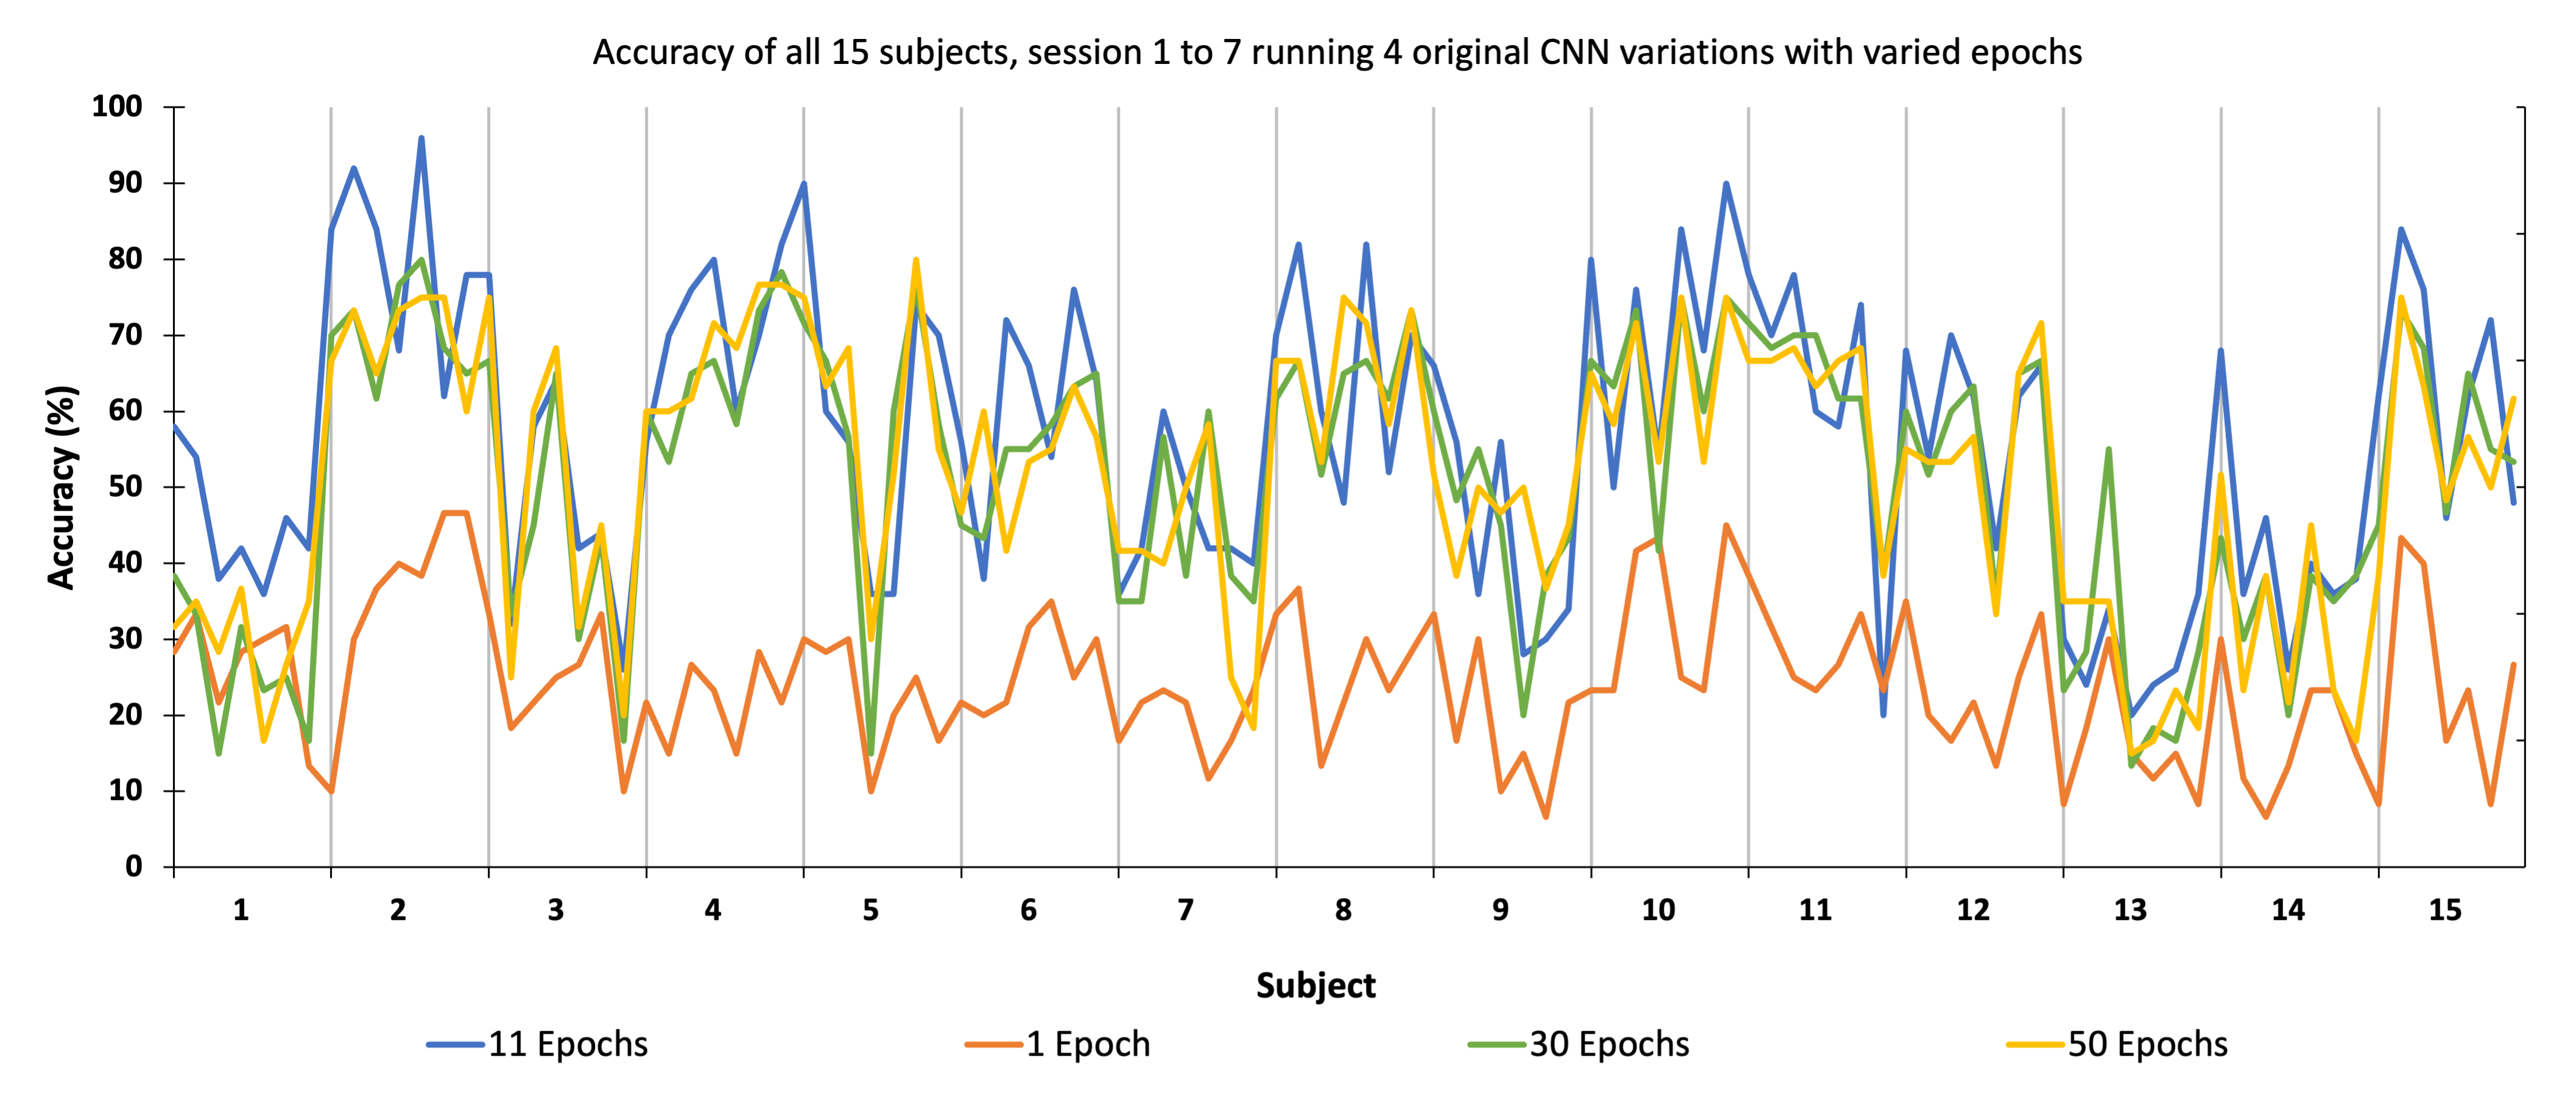
\includegraphics[scale=0.5]{Media/SBJ1-15_S1-7/SBJ1-15&S1-7_Varied_Epochs_Accuracy.png}
\caption{Best average test accuracy for all 105 sessions across all 15 subjects, comparing 4 runs of the CNN variation of 1, 11, 30 and 50 max epochs.}
\label{S1-7 Varied Epochs Acc}
\end{figure}

\subsection{Testing Epochs and Dropout Probabilities}
\label{All Subjects, 1 to 7 Testing Epochs and Dropout Probabilities SubSection}

Alongside altering the max epochs of the CNN, the dropout probabilities was raised all to 0.4\% to set more data to zero to further prevent over-fitting and then ran 3 variations with different epochs in \cref{S1-7 0.4 Dropout Varied Epoch Acc}. The accuracy's were 43.60\% at 1 epoch, 69.73\% at 11 epochs and 75.47\% at 30 epochs, this is lower than the original CNN variation, though was expected at more data is set to zero.

\begin{figure}[H]
\centering
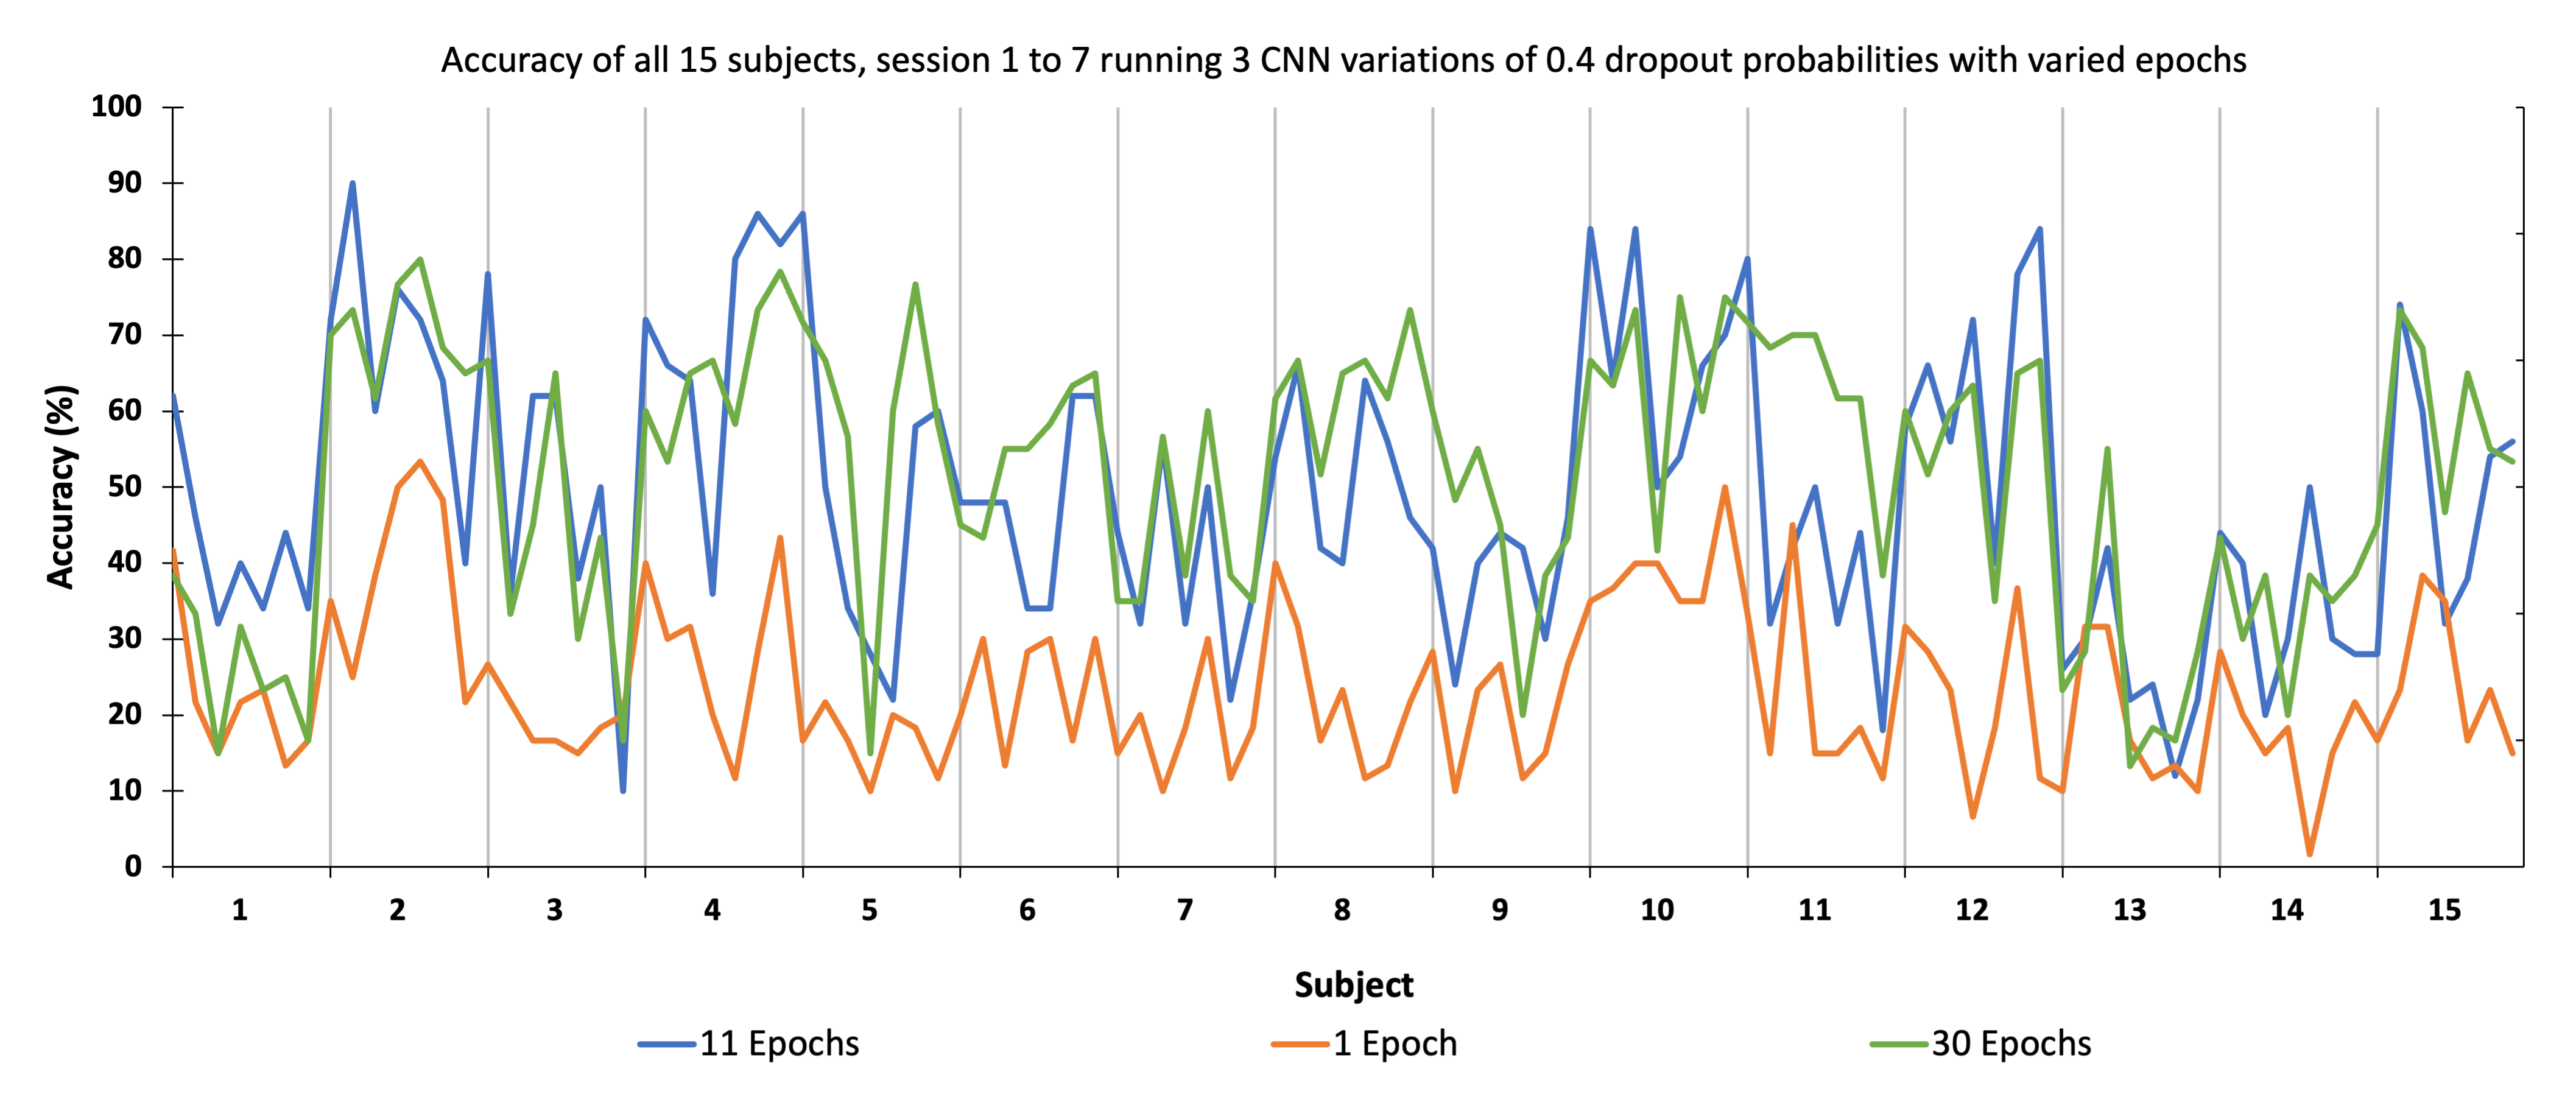
\includegraphics[scale=0.5]{Media/SBJ1-15_S1-7/SBJ1-15&S1-7_04_Dropout_Varied_Epochs_Accuracy.png}
\caption{Test accuracy for all 105 sessions across all 15 subjects, comparing 3 runs of the CNN variation of 0.4\% dropout probabilities and 1, 11 and 30 max epochs.}
\label{S1-7 0.4 Dropout Varied Epoch Acc}
\end{figure}

\subsection{Varying the Number of Filters}
\label{All Subjects, 1 to 7 Varying the Number of Filters SubSection}

Due to run time issues, these tests were only run once with 30 epochs however a baseline accuracy value for 30 epochs of the original CNN variation was formed of 78.94\%. Alongside a learning rate of 0.005, 0.1\% dropout probabilities, the number of filters of the 3 convolutional 2D layers were doubled and halved in \cref{S1-7 0.1dp 0.005lr 30epochs varied filters}. For the halved number of filters gave an accuracy of 80.27\%, double gave 82.13\% and the original number of filters gave 81.07\%. But adjusting the number of filters, it shows that increasing the number of filters improves the testing accuracy, this follows the logic of how CNN's work as the data is being filtered more and extracting more from the data.

\begin{figure}[H]
\centering
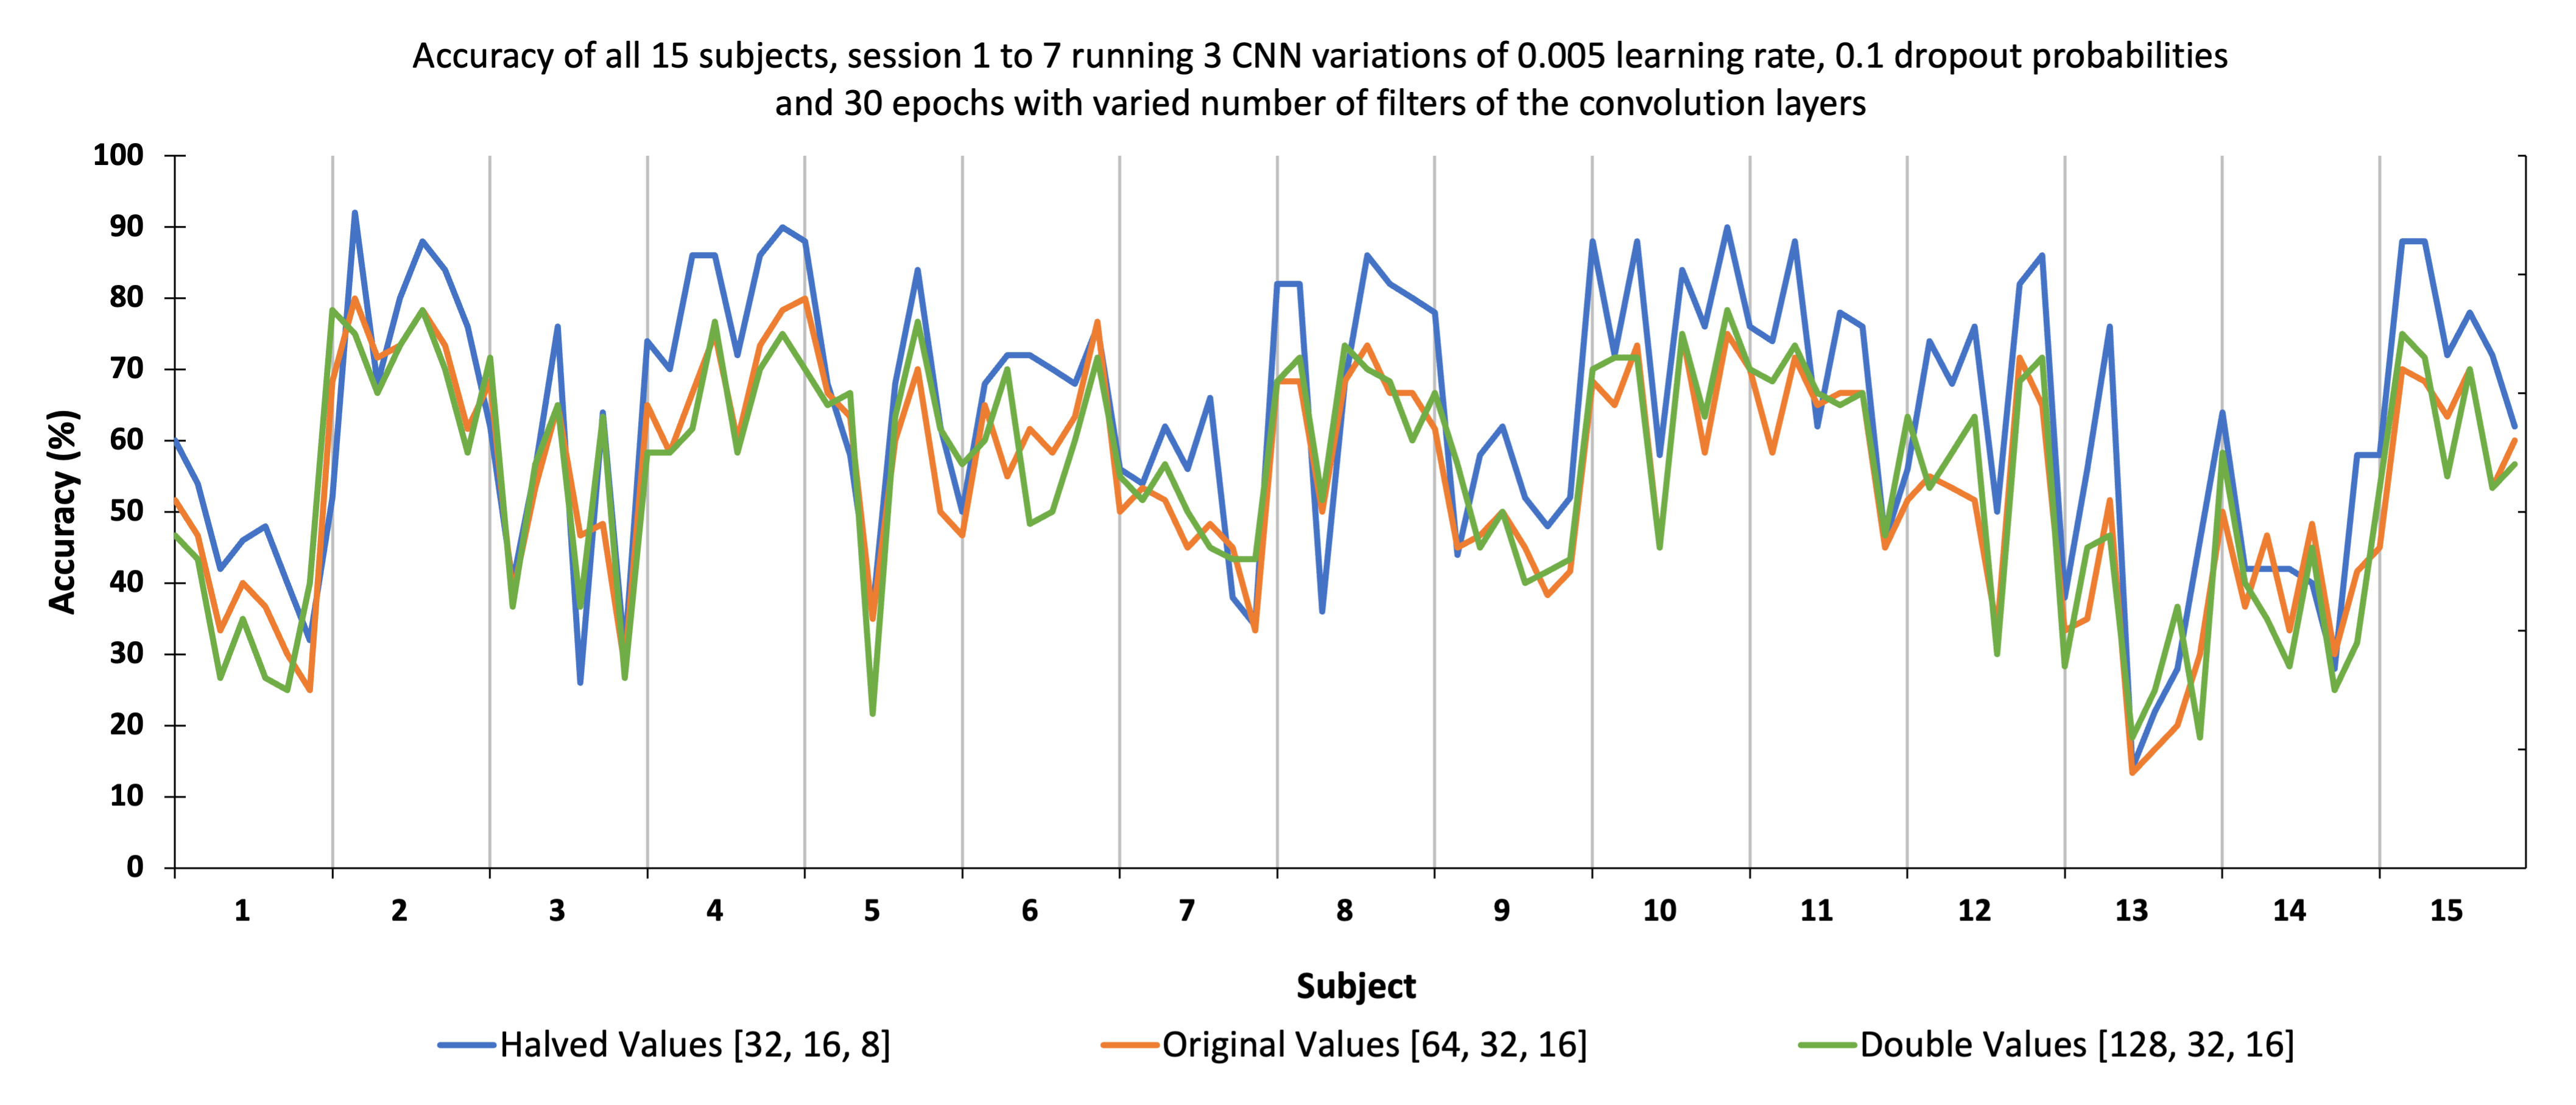
\includegraphics[scale=0.5]{Media/SBJ1-15_S1-7/SBJ1-15&S1-7_Varied_Filter_Numbers_Accuracy.png}
\caption{Test accuracy for all 105 sessions across all 15 subjects, comparing 3 runs of the CNN variation with 0.005 initial learning rate, 0.1\% dropout probabilities, 30 max epochs and varied number of filters in the convolutional layers.}
\label{S1-7 0.1dp 0.005lr 30epochs varied filters}
\end{figure}

\subsection{Varying the Fully Connected Layer}
\label{All Subjects, 1 to 7 Changing the Epochs SubSection}

The fully connected layer is the last 2 full layers, which dictates the dimensions of the data through its output size, by adjusting this proved that lowering the output size increased the accuracy \cref{S1-7 0.005lr 0.1dr 30epoch varied fcl}. By using 0.005 learning rate, 0,1\% learning rate and 30 max epochs with the original and halved values for the output size gave accuracy's of 81.20\% and 83.87\% respectively. By lowering the output size of the fully connected layer, the data is effect more by the weights and biases of the CNN, which is calculated automatically leading to high valued data being outputted.

\begin{figure}[H]
\centering
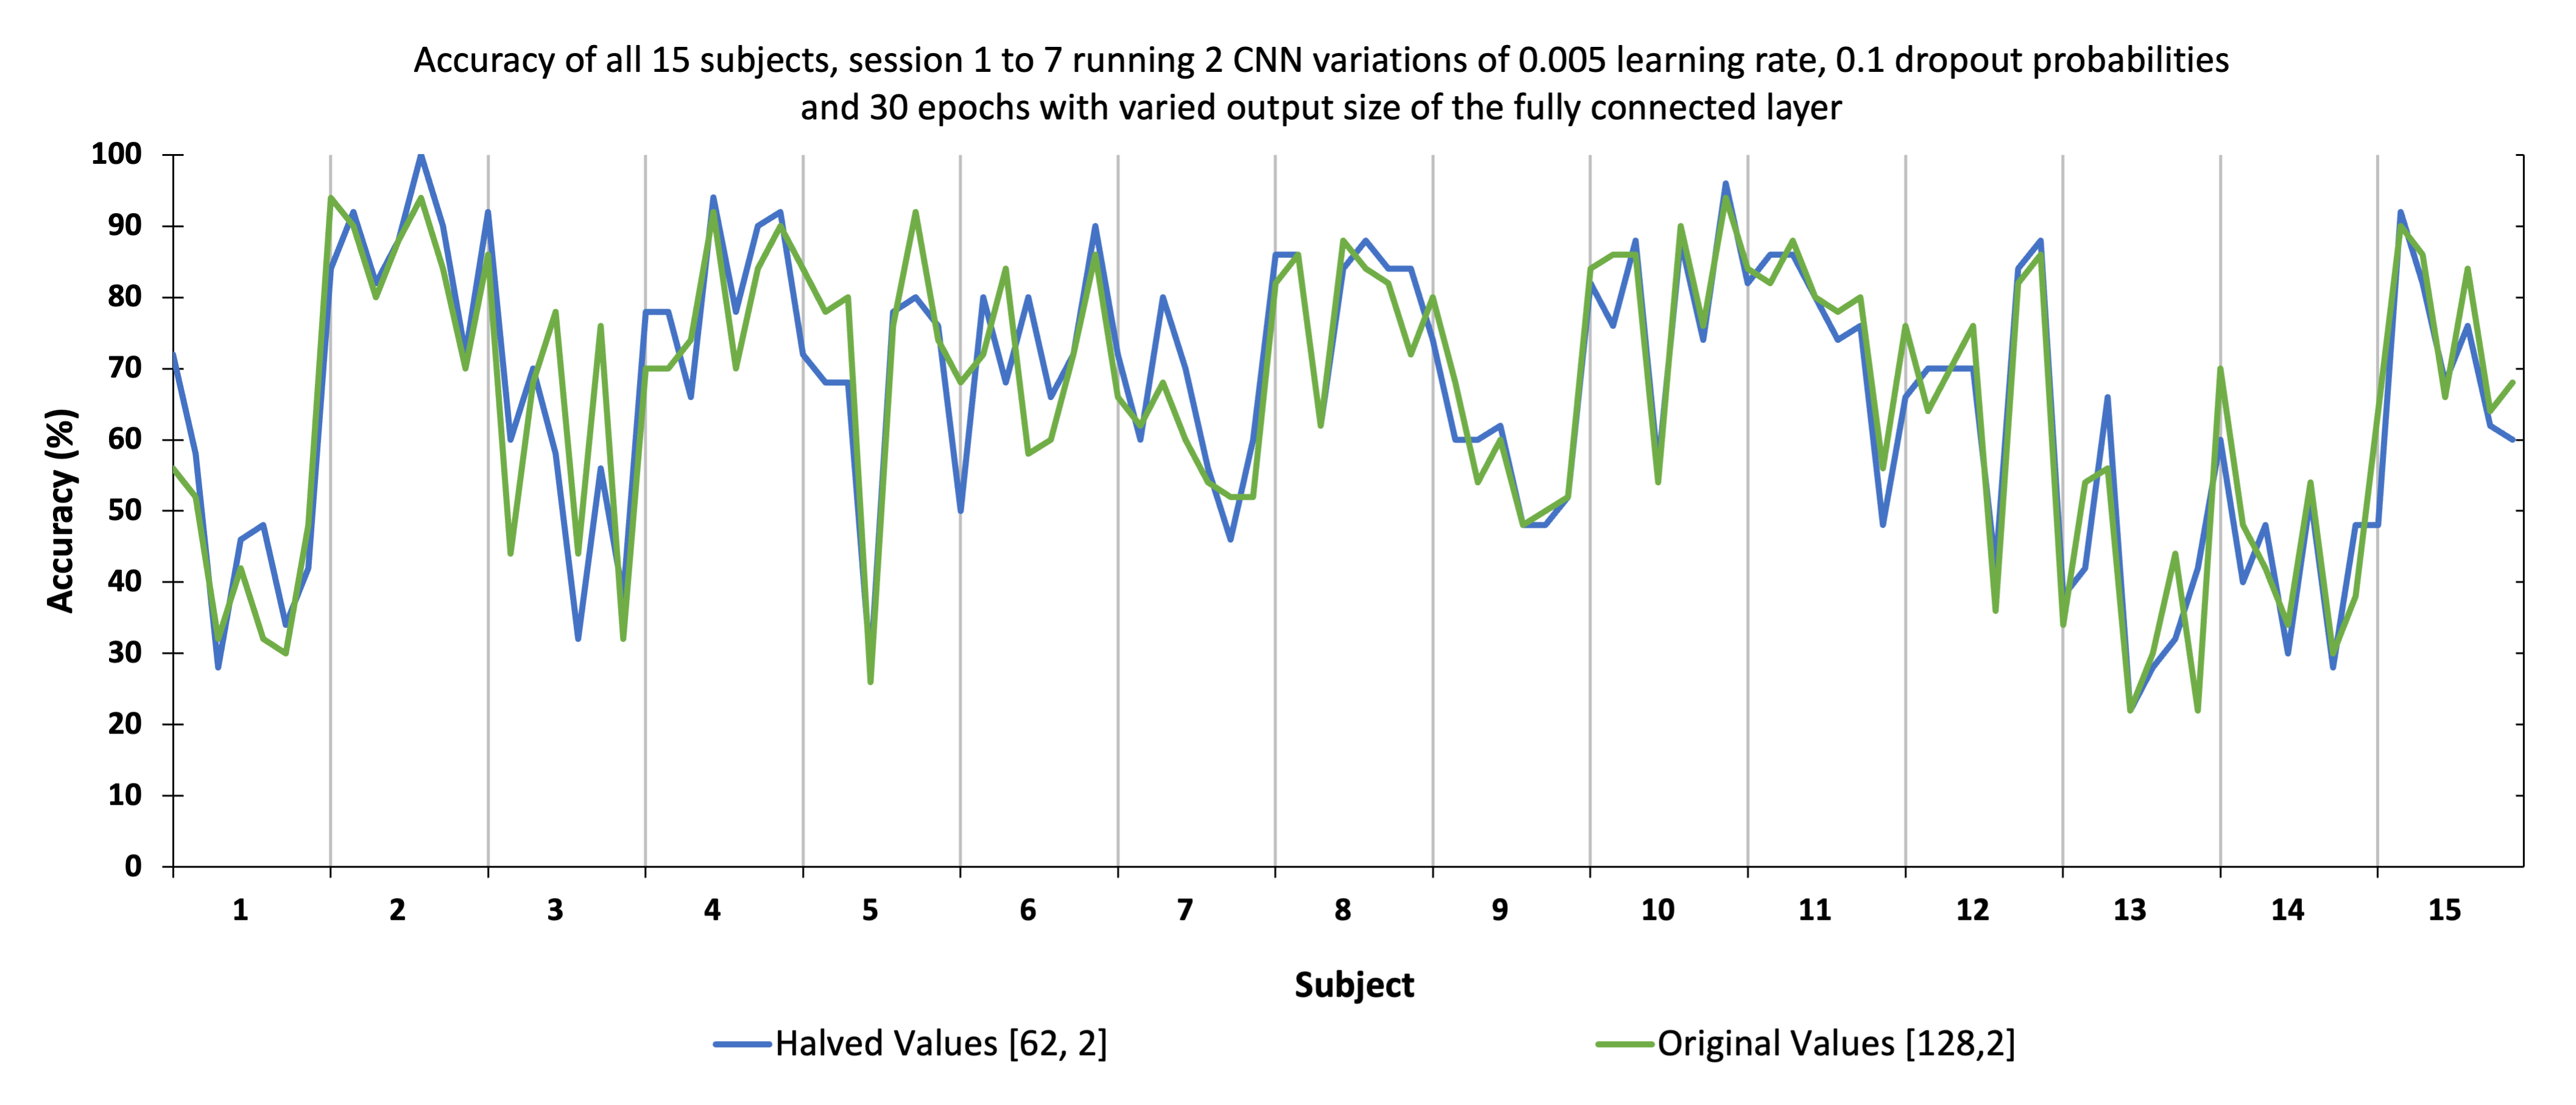
\includegraphics[scale=0.5]{Media/SBJ1-15_S1-7/SBJ1-15&S1-7_Varied_FullyConnctedLayer_Accuracy.png}
\caption{Test accuracy for all 105 sessions across all 15 subjects, comparing 2 runs of the CNN variation with 0.005 initial learning rate, 0.1\% dropout probabilities, 30 max epochs and varied output size of the fully connect layer.}
\label{S1-7 0.005lr 0.1dr 30epoch varied fcl}
\end{figure}

\subsection{Testing Multiple Features}
\label{All Subjects, 1 to 7 Testing Multiple Features SubSection}

\begin{figure}[H]
\centering
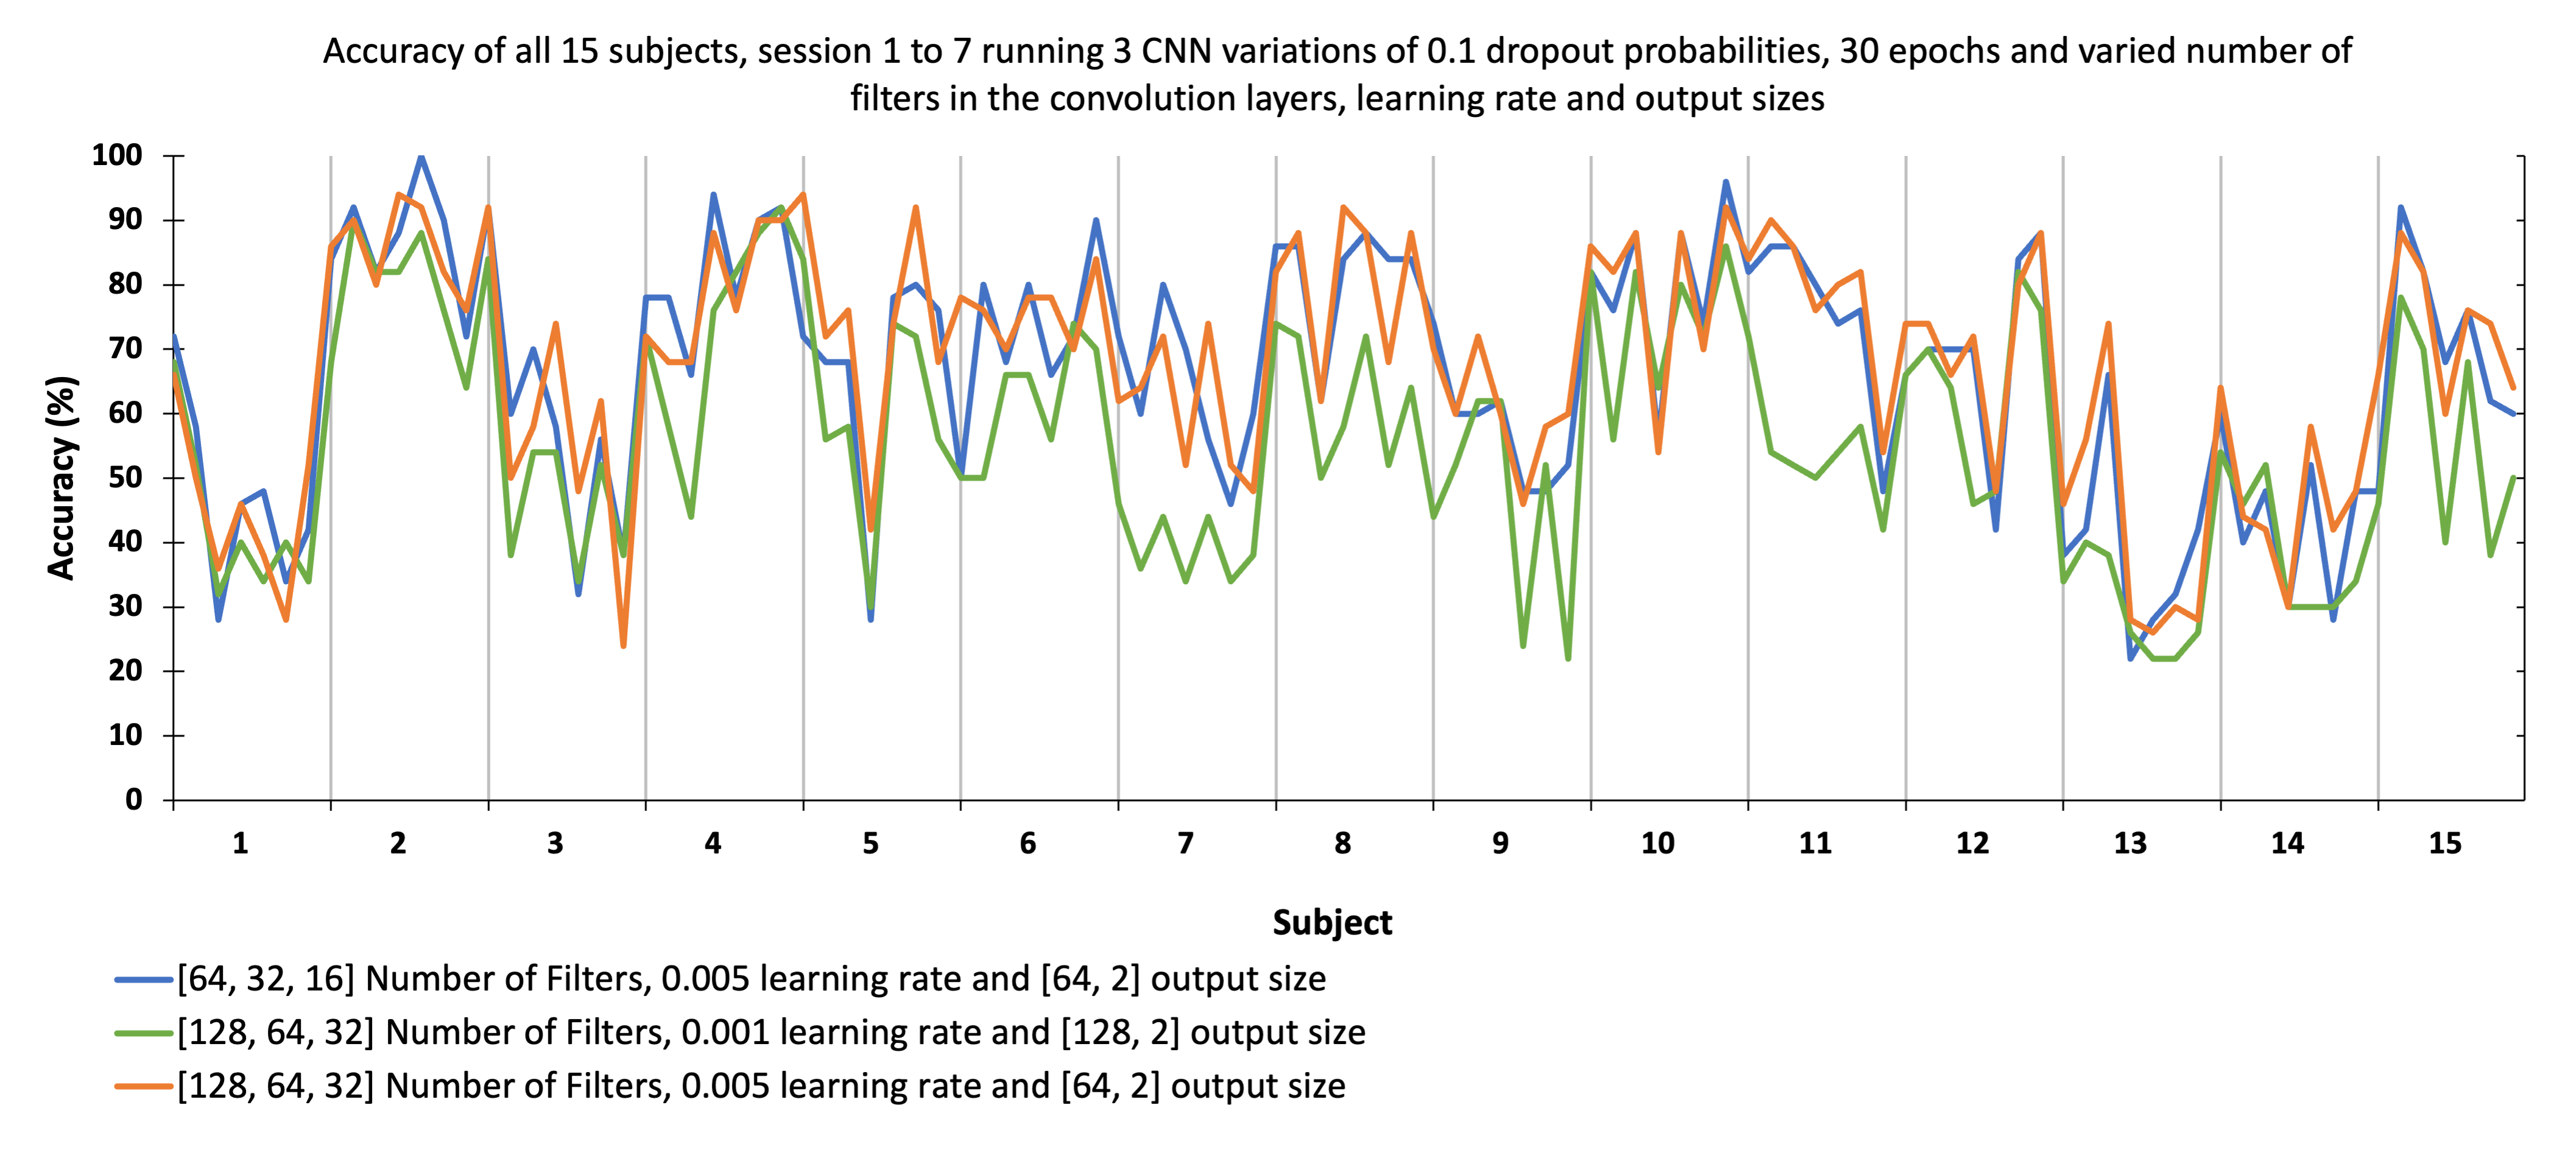
\includegraphics[scale=0.5]{Media/SBJ1-15_S1-7/SBJ1-15&S1-7_Varied_No_Of_Filters_and_Learning_Rate_Accuracy.png}
\caption{Test accuracy for all 105 sessions across all 15 subjects, comparing 2 runs of the CNN variation with 0.1\% dropout probabilities, 30 max epochs, varied number of filters and initial learning rates.}
\label{S1-7 0.1dr varied filters 30 epochs varied lr}
\end{figure}

In \cref{S1-7 0.1dr varied filters 30 epochs varied lr} set the dropout probabilities to 0.1\%, 30 max epochs with varied number of filters, learning rates and output sizes of the fully connected layer. With a 0.001 learning rate, doubled number of filters and original output sizes tested at 72.40\%. For double number of filters, 0.005 learning rate and half the original output size, tested for 83.60\% while the best result out of this project came from keeping the original number of filters, 0.005 learning rate and halving the output size with a test accuracy of 83.87\%. The dropout layer was also placed after the max pooling layer which allows the downsampling to occur before values are set to zero using the dropout layer, which is lowered in probability. This design of the CNN proved to be the most successful.

\section{All Subjects, Session 1 to 3 Classification}
\label{All Subjects, Session 1 to 3 Classification Section}

\begin{figure}[H]
\centering
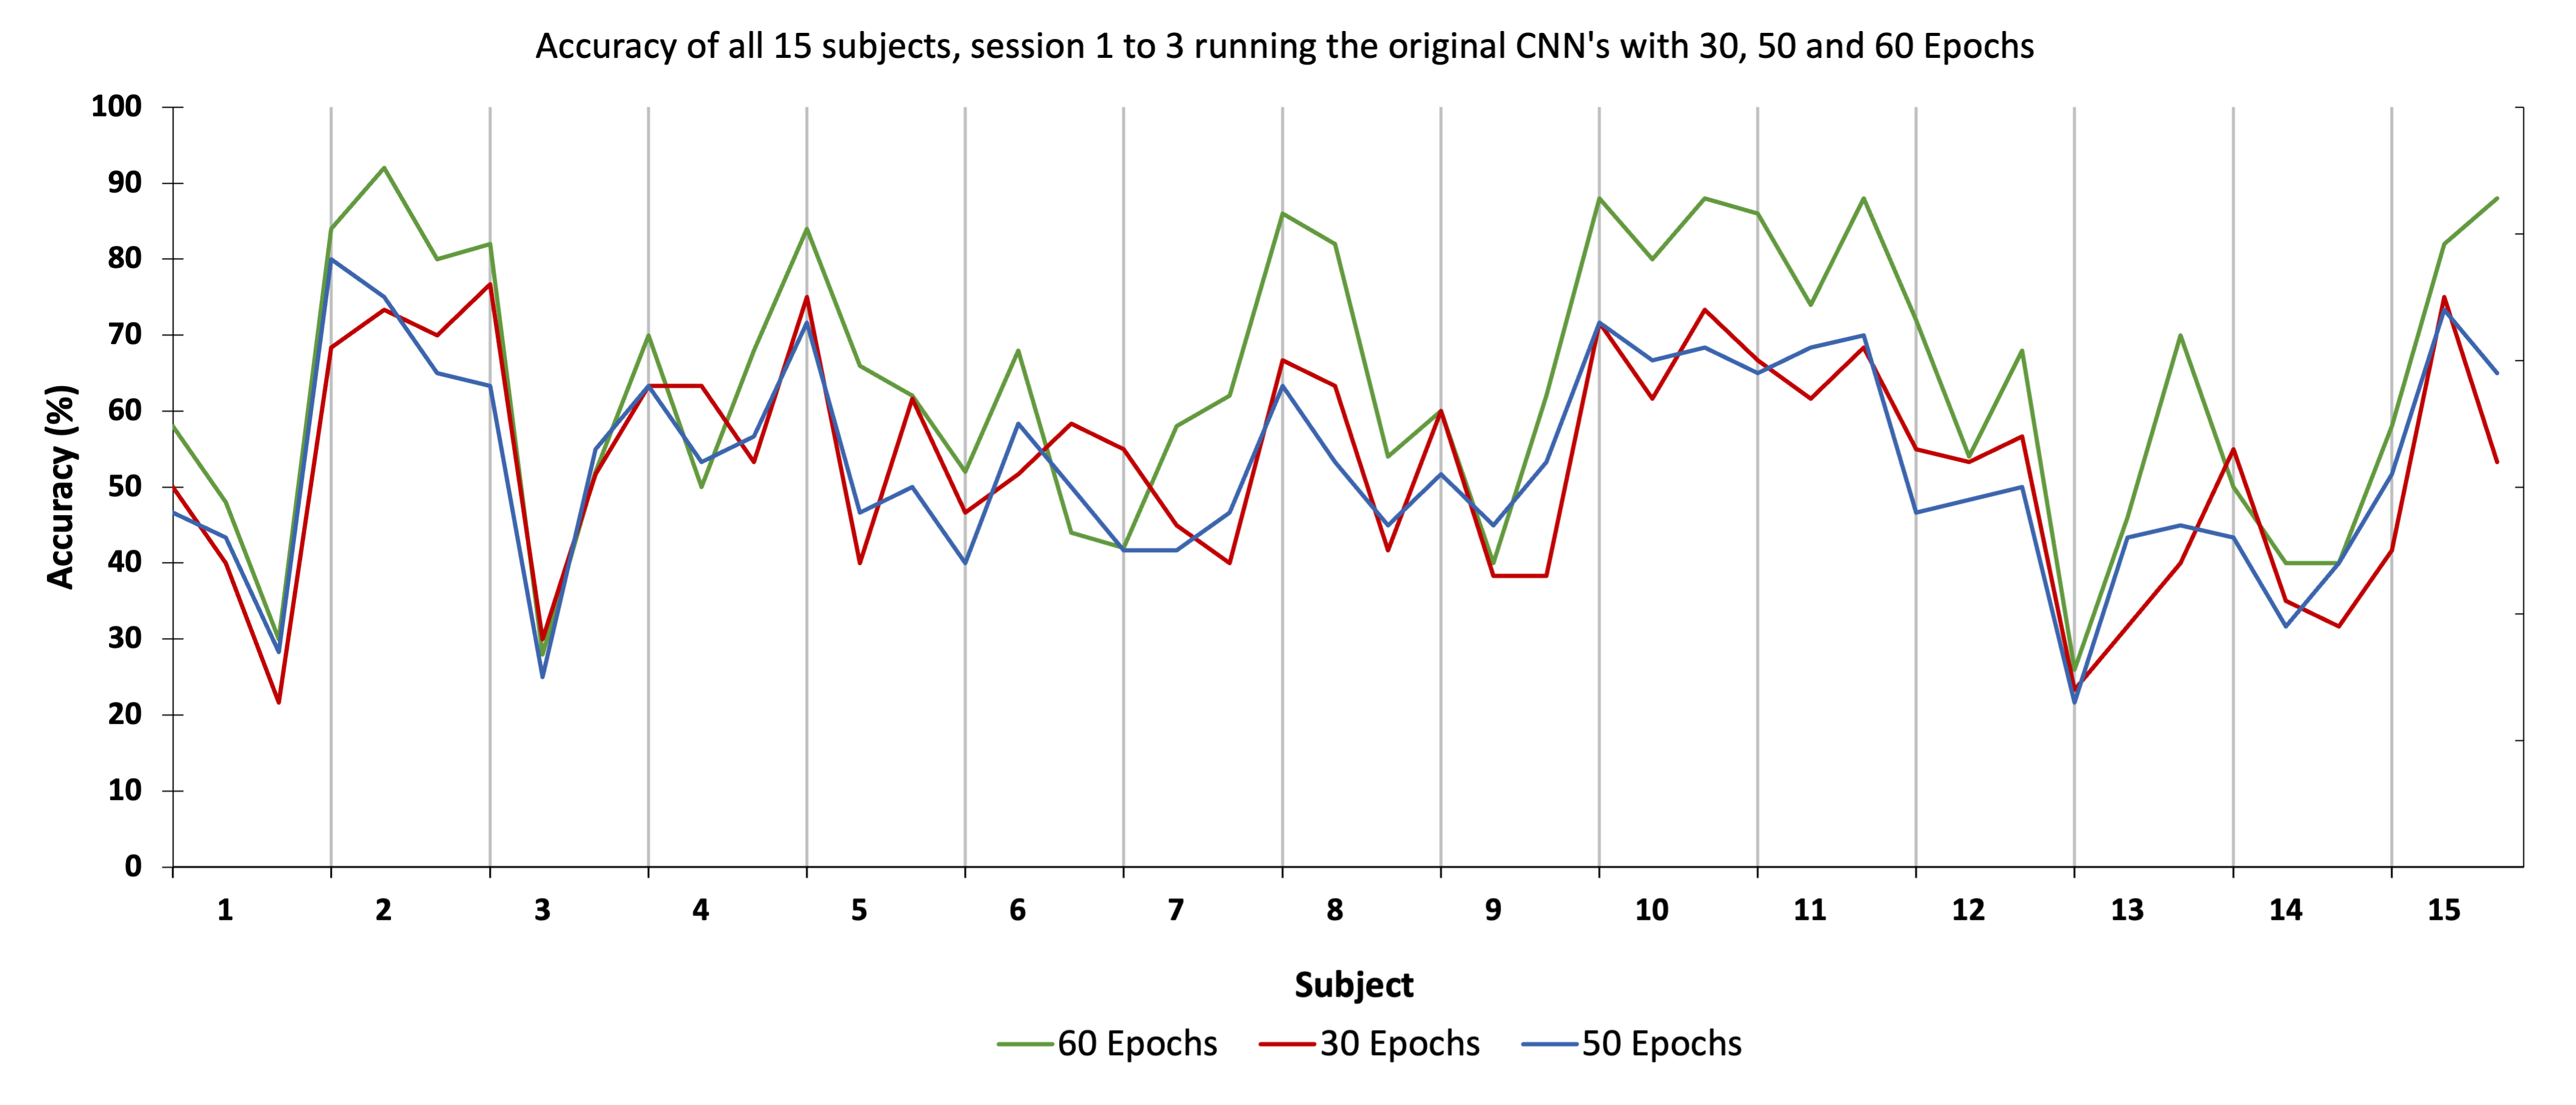
\includegraphics[scale=0.5]{Media/SBJ1-15_S1-3/SBJ1-15&S1-3_30&50_Epochs_Accuracy.png}
\caption{Test accuracy for all 45 sessions across all 15 subjects, sessions 1 to 3, comparing 3 runs of the CNN variation with 30, 50 and 60 max epochs}
\label{S1-3 30 50 epochs}
\end{figure}

\begin{figure}[H]
\centering
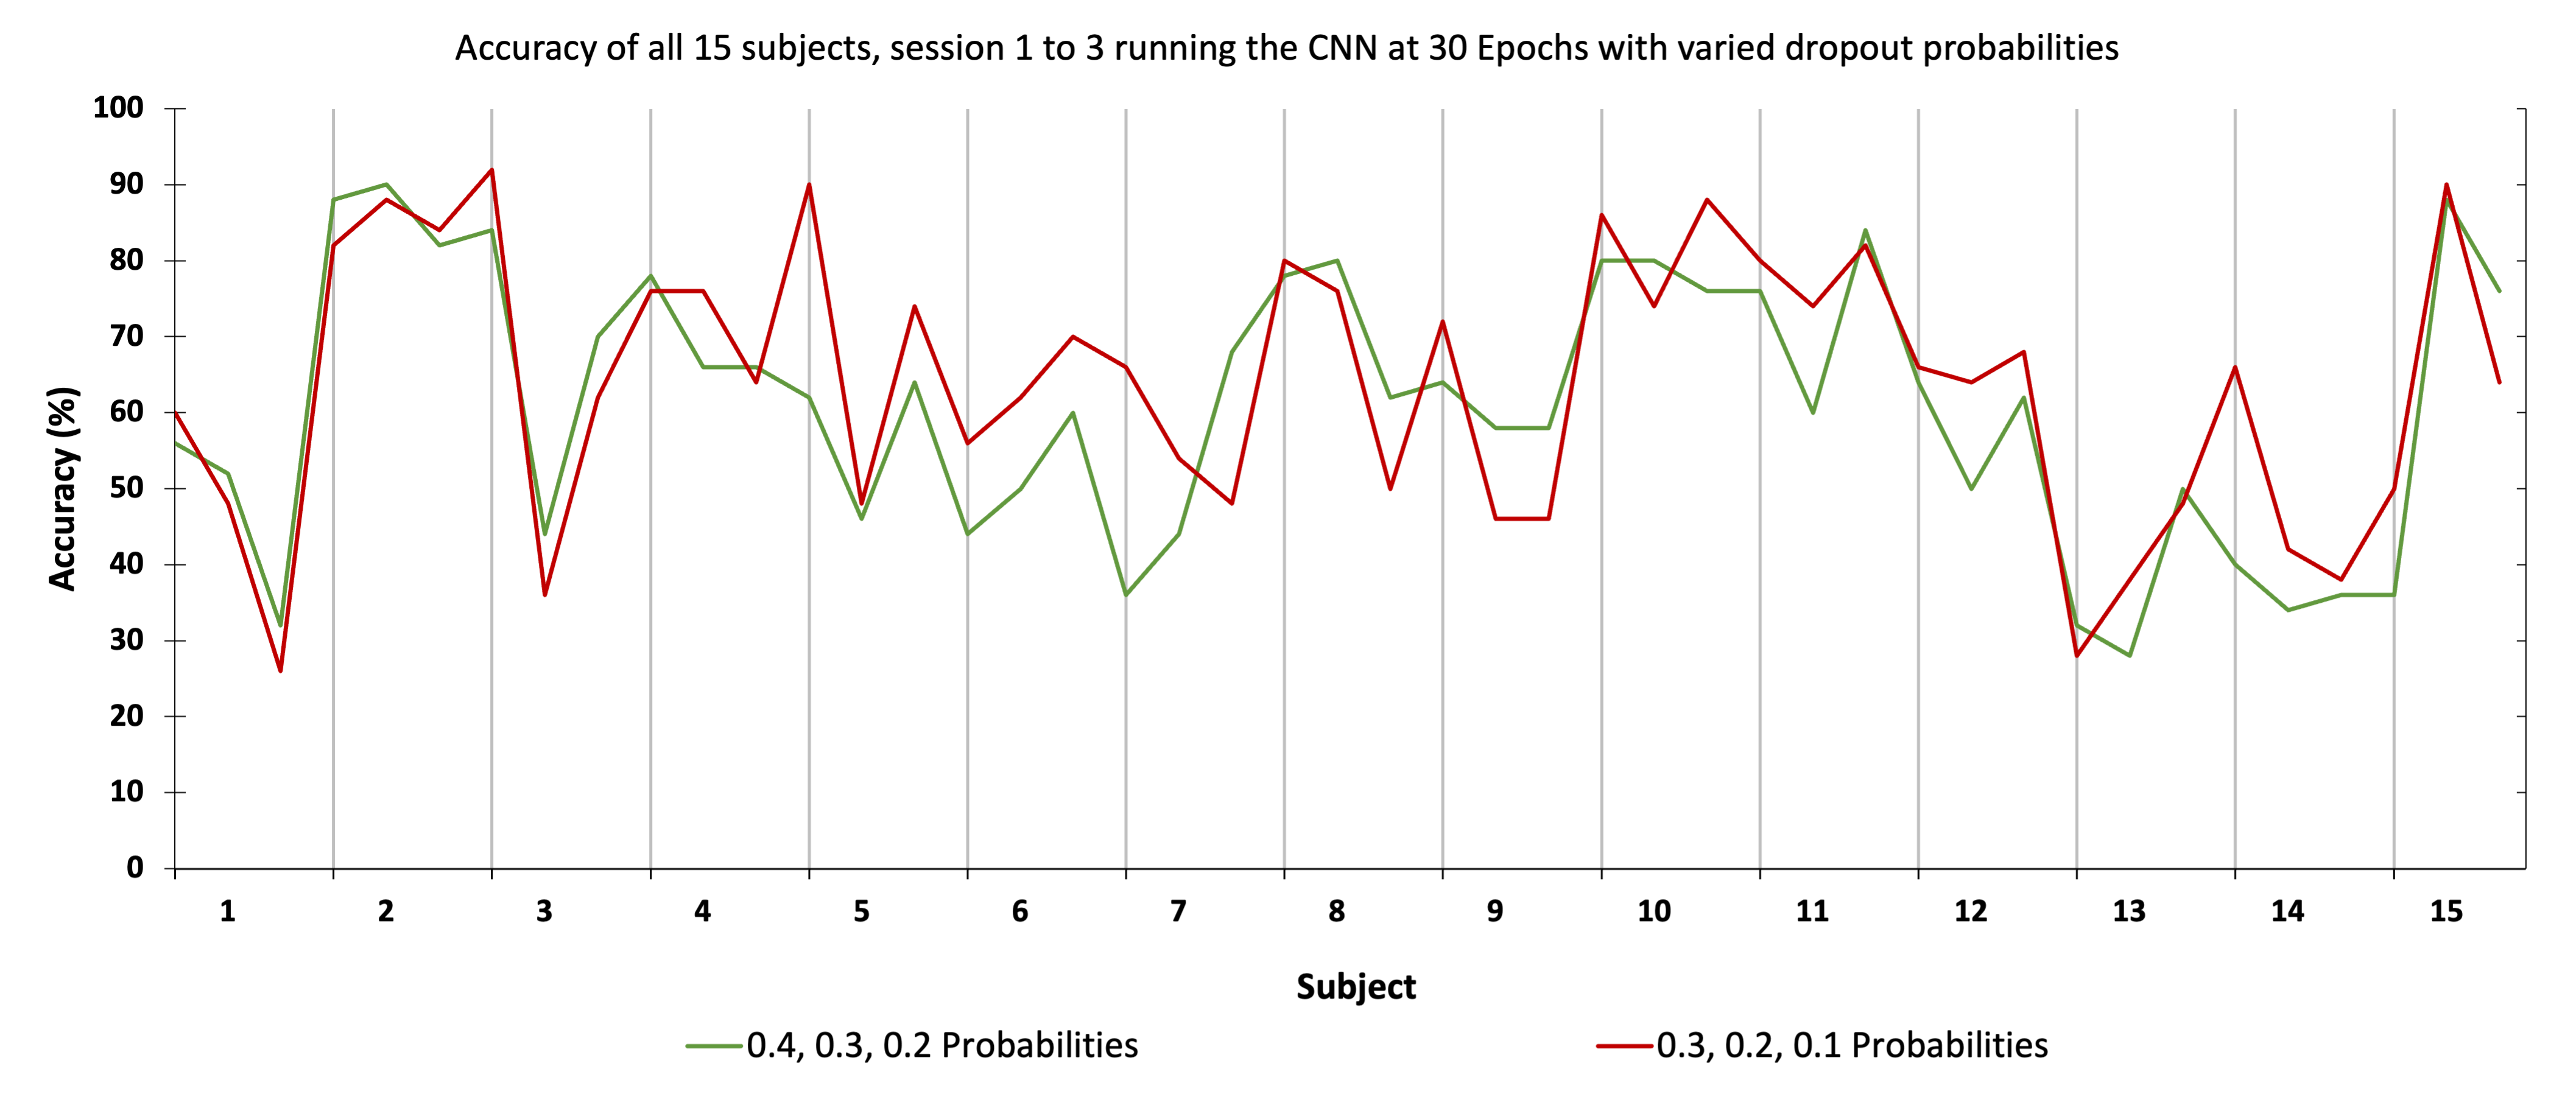
\includegraphics[scale=0.5]{Media/SBJ1-15_S1-3/SBJ1-15&S1-3_30_Epochs_Varied_Dropout_Accuracy.png}
\caption{Test accuracy for all 45 sessions across all 15 subjects, sessions 1 to 3, comparing 2 runs of the CNN variation with 30 max epochs and varied dropout probabilities.}
\label{S1-3 30 epochs varied dr}
\end{figure}

In an attempt to replicate the phase 1 of \cite{DatasetPaper}, which no accuracy was provided, tested sessions 1 to 3. \cref{S1-3 30 50 epochs} shows 60, 50 and 30 epoch variations of the original CNN being run for session 1 to 3. 60 epochs with 74.67\%, 50 epochs with 78.27\% and 30 epoch with 75.73\%. With run time for 50 and 60 epoch even with smaller data, the test continued with 30 epoch as further experimentation of dropout probabilities occurred in \cref{S1-3 30 epochs varied dr}, the original CNN variation gave a 75.73\% accuracy with [0.3, 0.2, 0.1] as the dropout probabilities and when all 3 dropout layers increased by 0.1 gave 70\%. The final test on session 1 to 3 was varying the number of filters at 30 epochs with 0.005 learning rate in \cref{S1-3 30 epochs varied filters}, gave the original number of filters an accuracy of 78.13\% and halving the number of filters gave an accuracy of 75.73\%.

\begin{figure}[H]
\centering
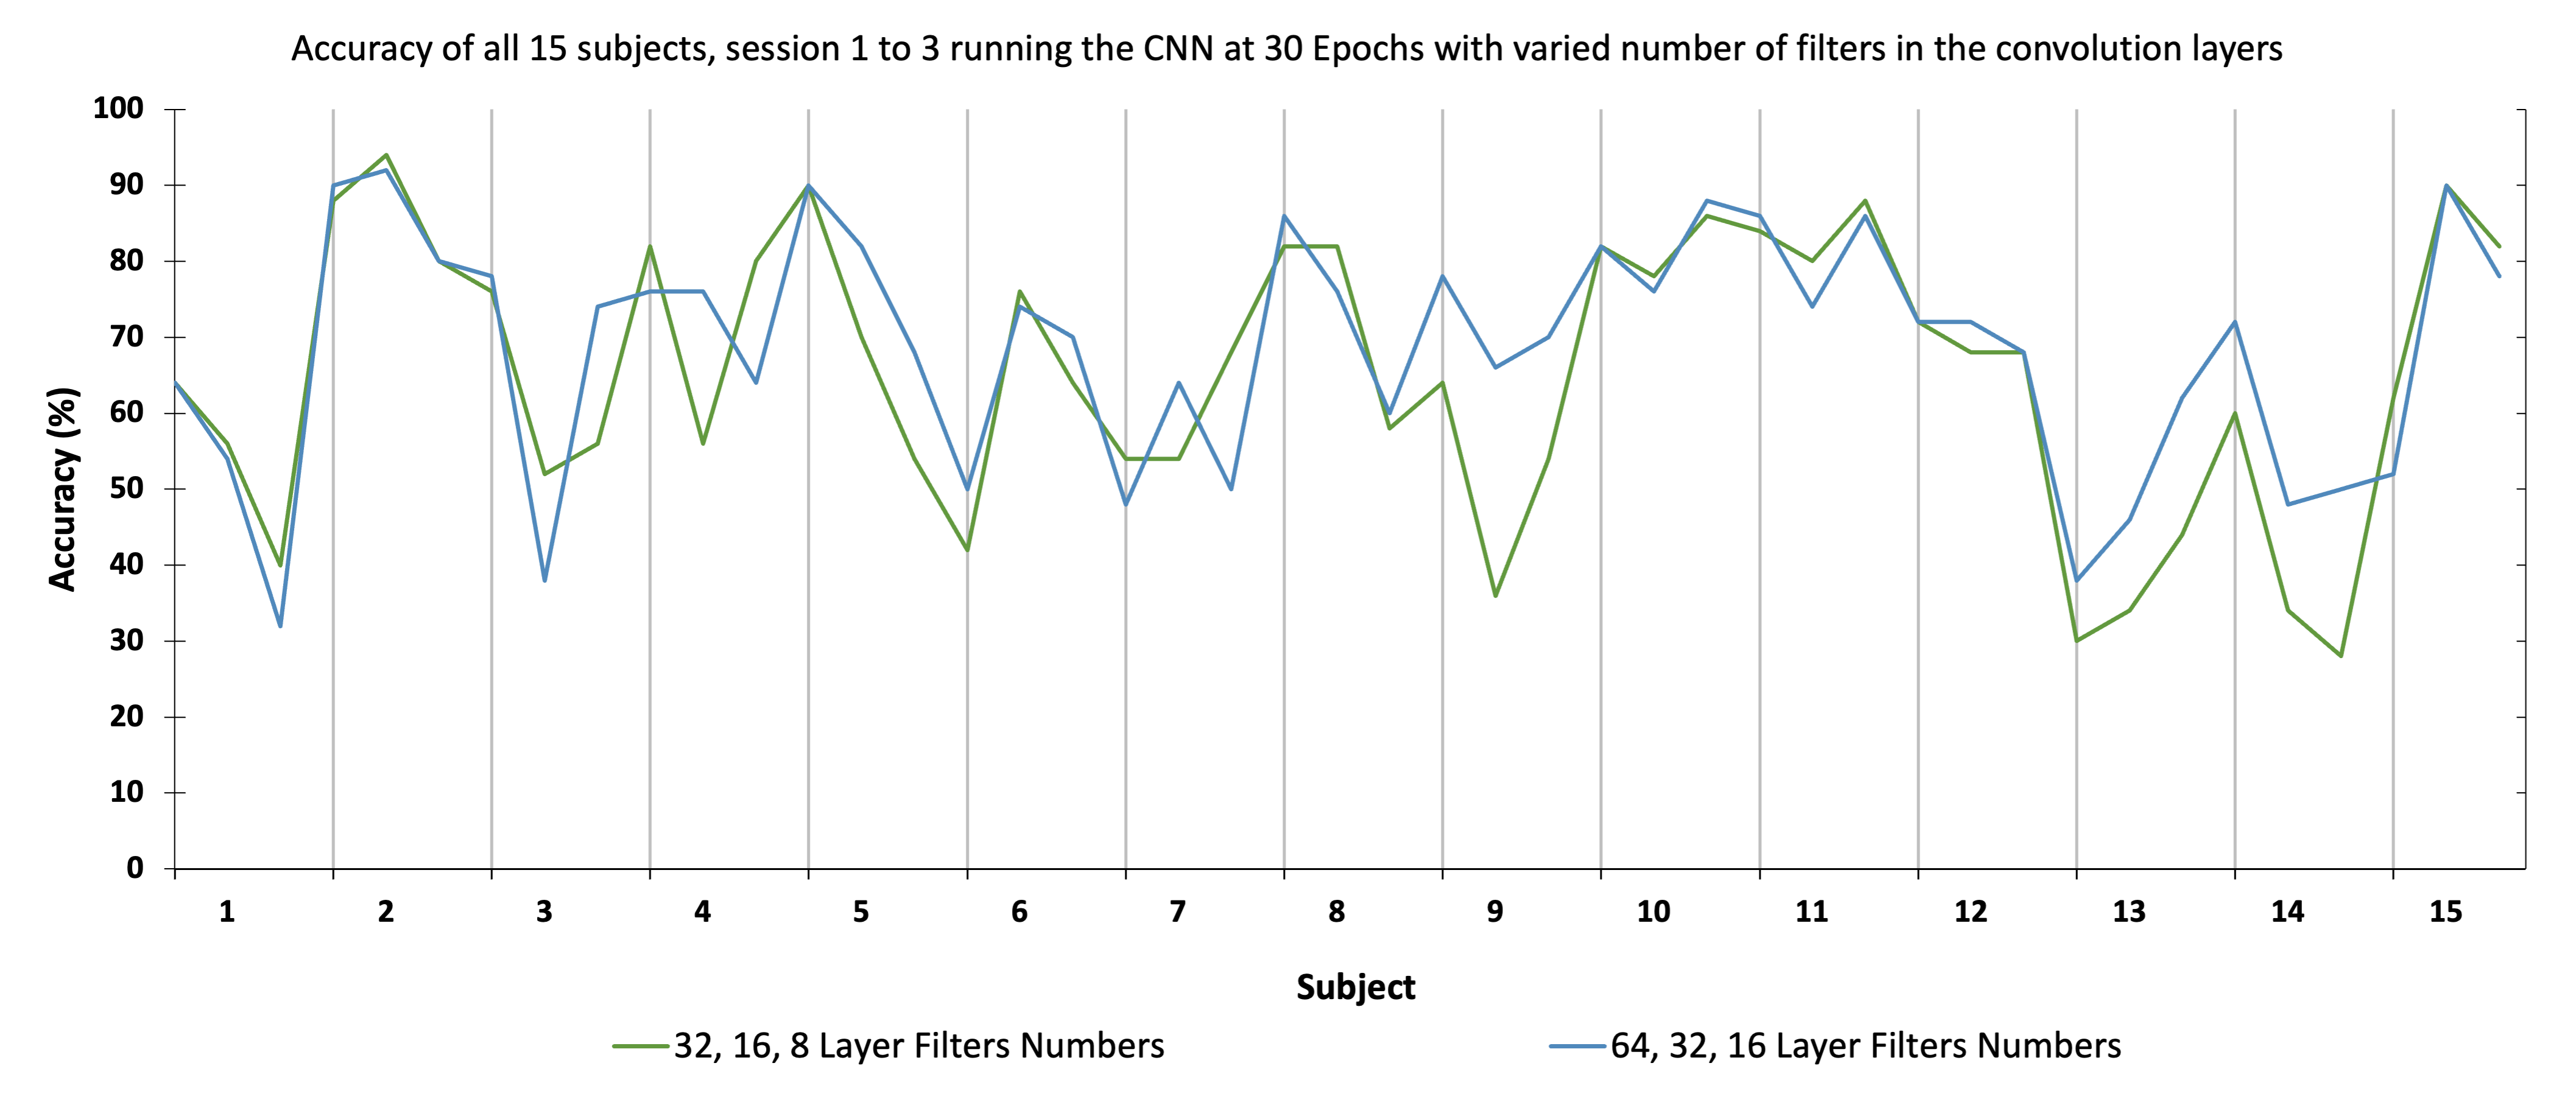
\includegraphics[scale=0.5]{Media/SBJ1-15_S1-3/SBJ1-15&S1-3_30_Epochs_Varied_No_Of_Filters_Accuracy.png}
\caption{Test accuracy for all 45 sessions across all 15 subjects, sessions 1 to 3, comparing 2 runs of the CNN variation with 30 max epochs and varied number of filters.}
\label{S1-3 30 epochs varied filters}
\end{figure}

\section{All Subjects, Session 4 to 7 Classification}
\label{All Subjects, Session 4 to 7 Classification Section}

\subsection{Testing Multiple Features}
\label{All Subjects, 4-7 Multiple Features SubSection}

An accuracy of 67\% was given for sessions 4 to 7 by \cite{PalaniPaper}. Utilising the features found beneficial to improve the accuracy in experimentation do with session 1-7, the epoch values were changed while keeping the initial learning rate at 0.005 and 0.1\% dropout probabilities but failed to improve upon the objective accuracy. As seen in \cref{S4-7 varied epochs}, 50 epochs: 63.8\%, 30 epochs: 63.42\%, 20 epochs: 71.4\% and 11 epochs: 52\%. The 50 epochs was run again using the original CNN variation as shown in \cref{S4-7 50 epochs vary dr lr} and gave a accuracy of 58.67\%. Analysis of which session yield better results indicates session 4 - 7 to be superior, benefited by an additional session. 

\begin{figure}[H]
\centering
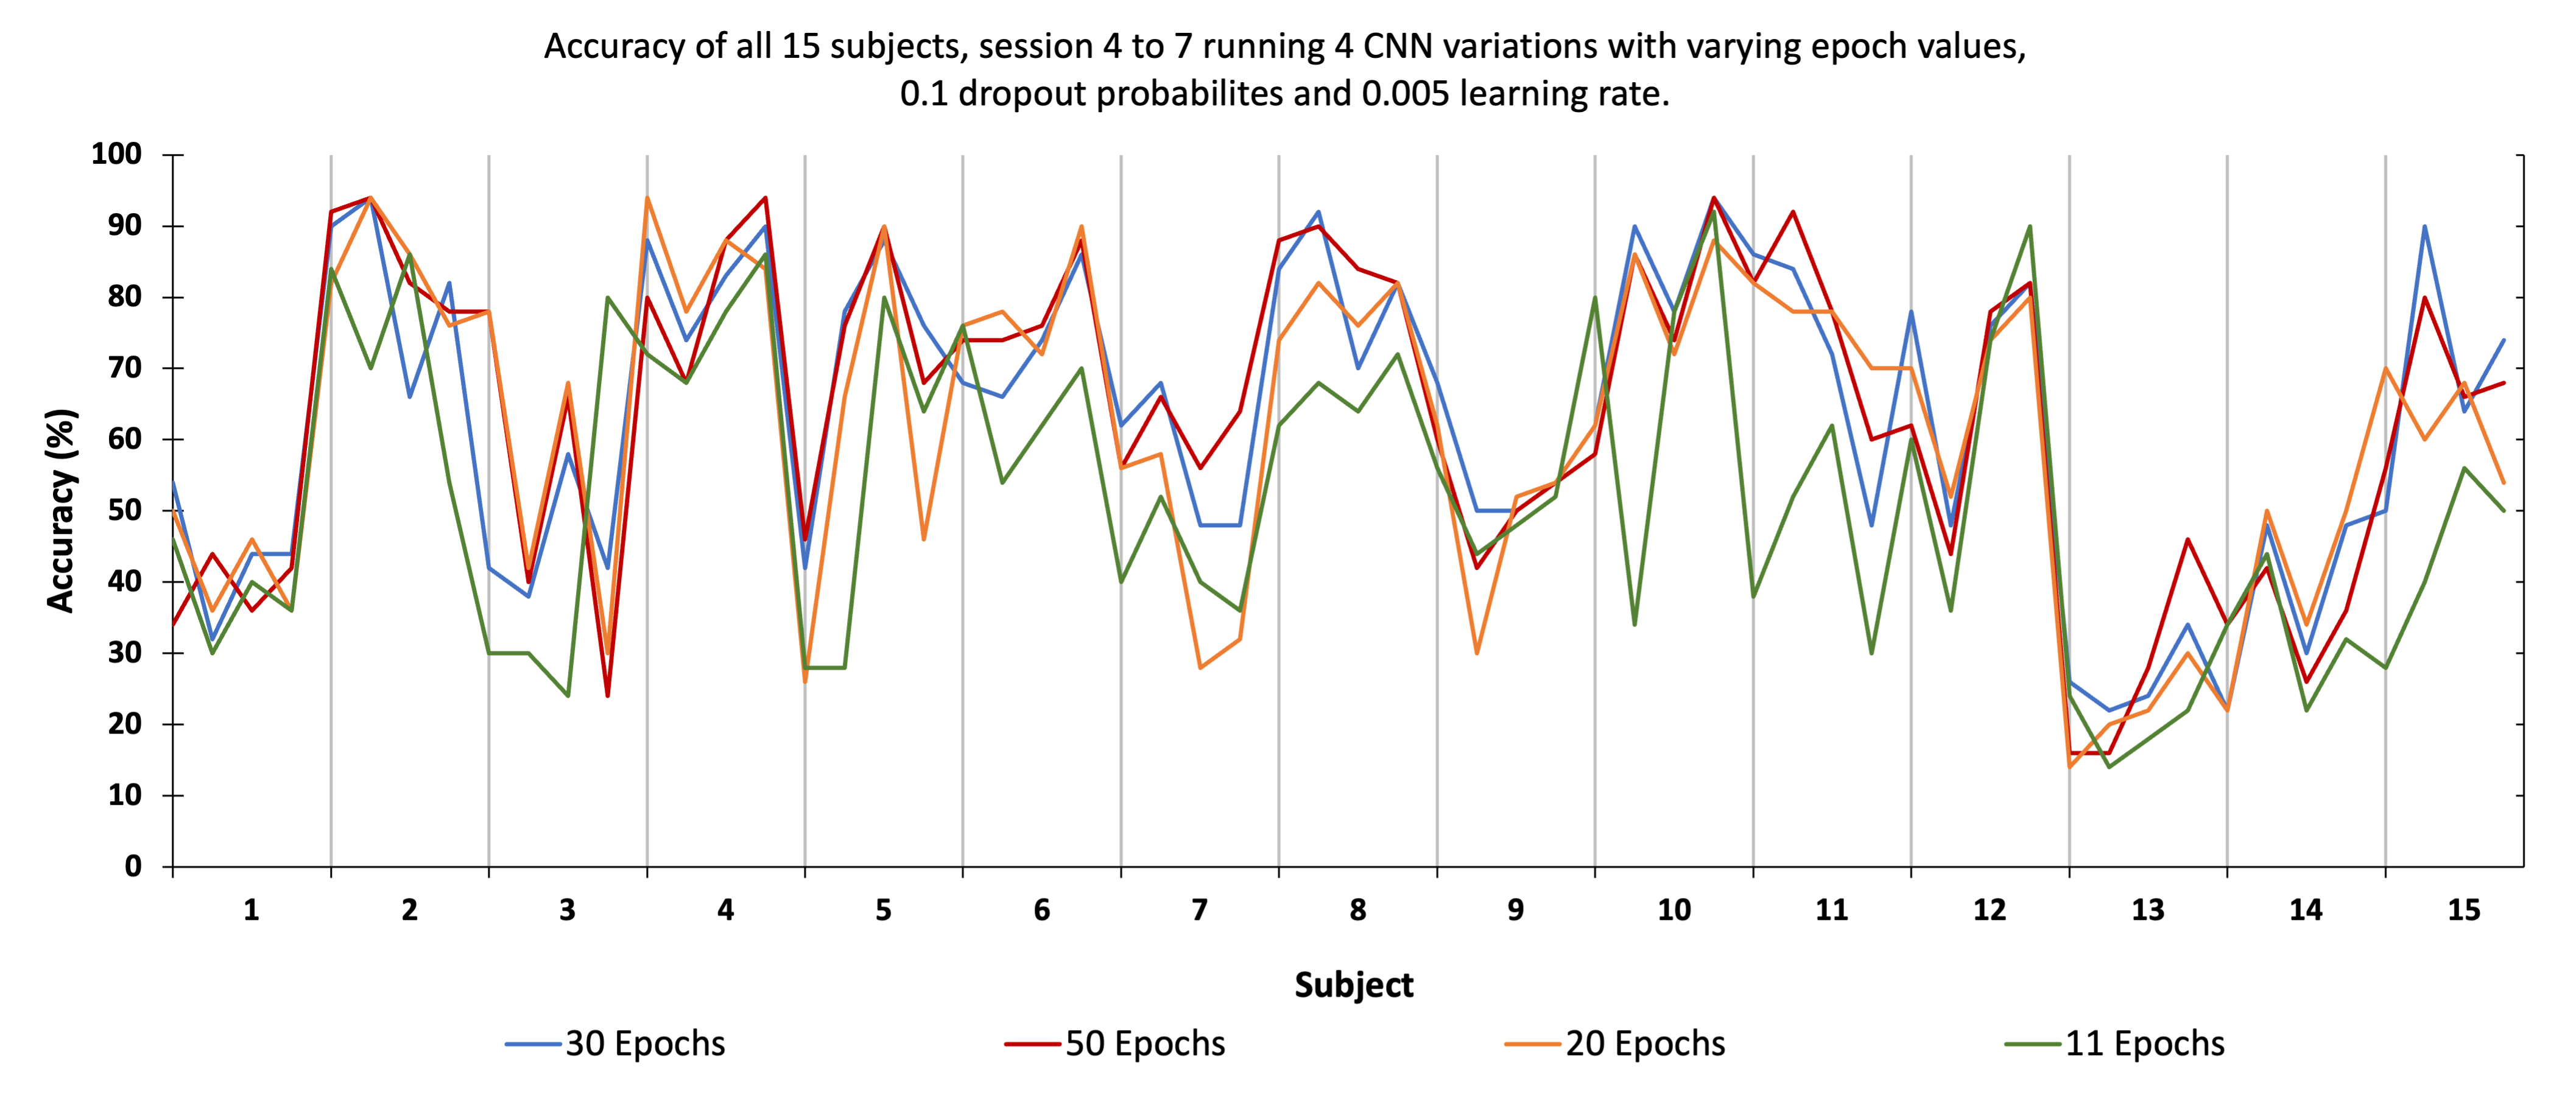
\includegraphics[scale=0.5]{Media/SBJ1-15_S4-7/SBJ1-15&S4-7_30&50&20&11_Epochs_Accuracy.png}
\caption{Test accuracy for all 60 sessions across all 15 subjects, sessions 4 to 7, comparing 4 runs of the CNN variation with 0.1\% dropout probabilities, 0.005 learning rate and varying max epochs.}
\label{S4-7 varied epochs}
\end{figure}

\begin{figure}[H]
\centering
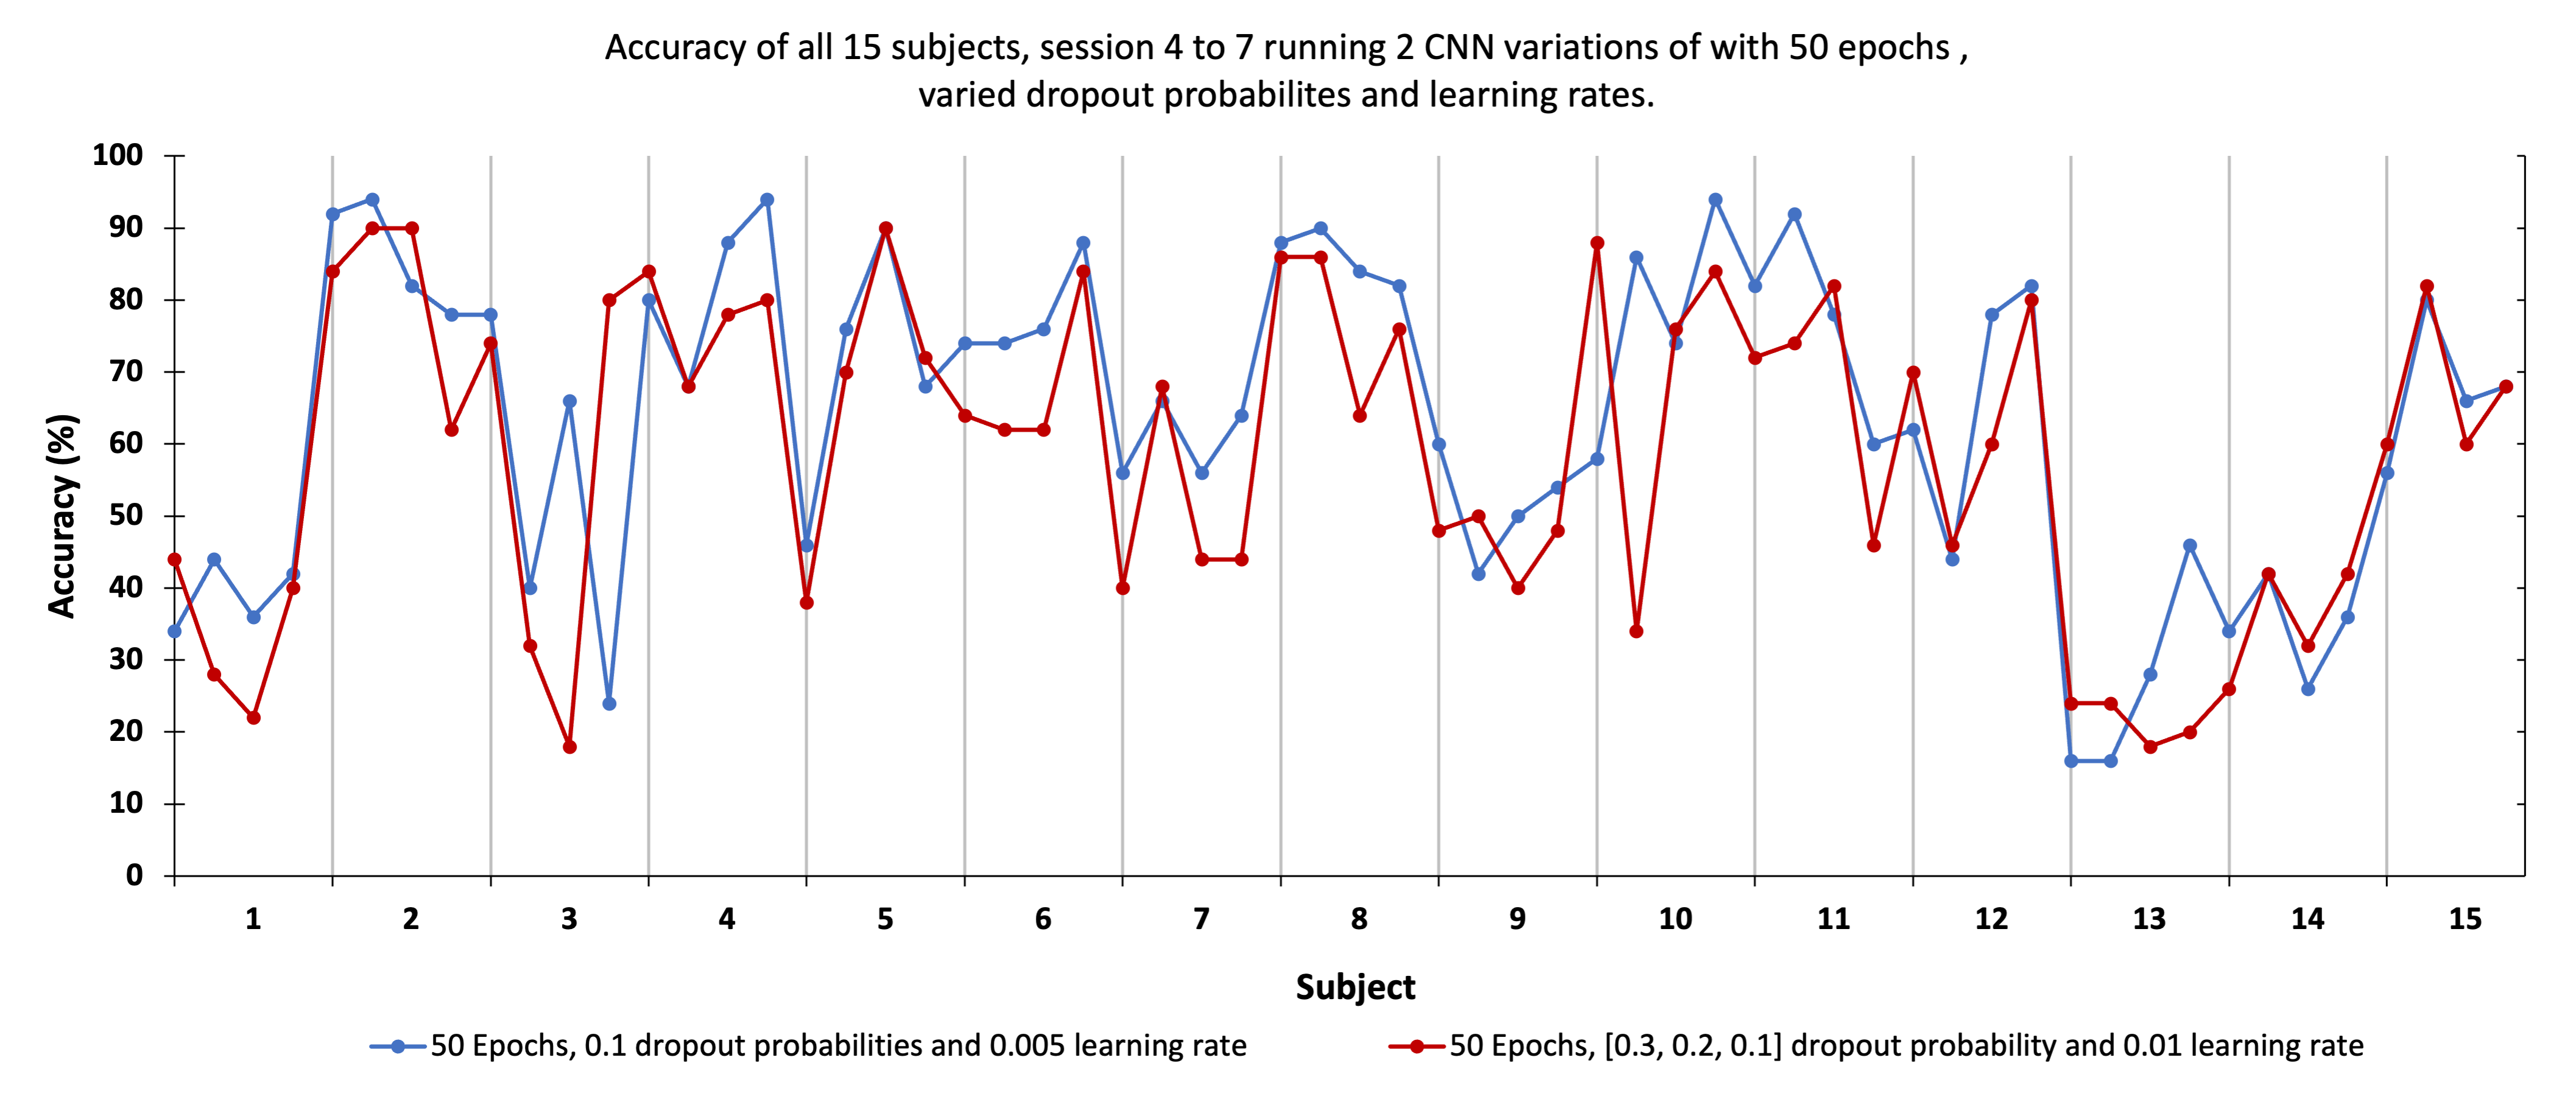
\includegraphics[scale=0.5]{Media/SBJ1-15_S4-7/SBJ1-15&S4-7_50_Epochs_Varied_Accuracy.png}
\caption{Test accuracy for all 60 sessions across all 15 subjects, sessions 4 to 7, comparing 2 runs of the CNN variation with 50 max epochs and varying dropout probabilities and learning rates.}
\label{S4-7 50 epochs vary dr lr}
\end{figure}

\section{Subject and Session Review}
\label{Subject and Session Review Section}

Observing the test accuracy for all the subjects and their sessions, it can be seen in every test that subjects: 2, 4, 8, 10 and 15 achieved high accuracy results within the data meaning these subject hold a direct relationship with the overall accuracy. A linear relationship can also be spotted in the results as to how the subject reacted during the clinical trial, in \cref{S4-7 50 epochs vary dr lr} a positive linear relationship holds over subjects: 1, 3, 5, 6, 9, 10, 12, 13 and 14. This indicates that this subject underwent more severe P300 neural response that the other over the course of the trial. Whereas a negative linear relation holds over subject: 2, 4, 7, 8, 11 and 15 as the trial went on from session 4 to 7, they encountered less severe P300 responses.